\documentclass[12pt]{article}
\usepackage{polyglossia}
\usepackage{fontspec}
\usepackage[export]{adjustbox}
\usepackage{amsfonts, amsmath, amssymb}
\usepackage{bm}
\usepackage{breqn}
\usepackage{derivative}
\usepackage{empheq}
\usepackage[inline]{enumitem}
\usepackage{fancyhdr}
\usepackage{geometry}
\usepackage{graphicx}
\usepackage{kantlipsum}
\usepackage{lastpage}
\usepackage{linebreaker} % line-breaker algorithm in LuaLaTeX
\usepackage{lualatex-math} % Fixes for mathematics
\usepackage{mathtools}
\usepackage{microtype}
\usepackage{nicefrac}
\usepackage[hyperref]{ntheorem}
% \usepackage{phfqit} % Bra-ket notation
% \usepackage{physics}
\usepackage[inline]{showlabels}
% \usepackage{simples-matrices}
\usepackage{siunitx}
\usepackage{soul}
\usepackage{titling}
\usepackage{tabularray}
\usepackage{tasks}
\usepackage{xcolor}
\usepackage{xfrac}
\usepackage{xparse}
\usepackage{xspace}
\usepackage{hyperref}
% Polyglossia config
\setdefaultlanguage[variant=mexican]{spanish}
\setotherlanguage{english}
\usepackage{cleveref}

%%%%%%%%%%%%%%%%%%%%%%%%%%%%%%%%%%%%%%%%%%%%%%%%%%%%%%%%%%
%%%%%%%%%%%%%%%%%%%%%%%%%%%%%%%%%%%%%%%%%%%%%%%%%%%%%%%%%%
%%%%%%%%%%%%%%%%%%Configuraciones extras%%%%%%%%%%%%%%%%%%
\definecolor{base3}{RGB}{253, 246, 227}%
\definecolor{pinkwave}{RGB}{255, 0, 128}%
\definecolor{customBlue}{RGB}{11, 61, 98}%
\pagecolor{base3}
\graphicspath{{img/}}
\setlength{\parindent}{2em} % Sangría
\setlength{\parskip}{0.5em} % Espacio entre párrafos
\linespread{1.1} % line spacing
\setlength{\jot}{10pt} % Space between lines in multiline eqs
\crefname{equation}{ec.}{ecs.} % Equation's cross-reference name

% Line-breaker config
\linebreakersetup {
    maxtolerance = 90,
    maxemergencystretch = 1em,
    maxcycles = 4
}

%%%%%%%%%%%%%%%%%%Theorem environments%%%%%%%%%%%%%%%%%%
% Configuración de ambiente para problema
\theoremstyle{break}
\theoremheaderfont{\Large\normalfont\bfseries}
\theorembodyfont{\normalfont}
\theoremseparator{\bigskip} % Spacing between header and body
\theorempreskip{1.5em}
\theorempostskip{\topsep\bigskip}
\theorempostwork{
    \color{customBlue} \hrule width \hsize height 2pt \kern 1mm \hrule width \hsize
    }
\newtheorem{exercise}{Problema}
\counterwithin{equation}{exercise}

% Configuración de ambiente para solución
\theoremstyle{nonumberbreak}
\theoremheaderfont{\Large\normalfont\bfseries}
\theorembodyfont{\normalfont}
\theoremseparator{\medskip}
\theorempreskip{1em}
\theorempostskip{\topsep\medskip}
\newtheorem{solution}{Solución}

%%%%%%%%%%%%%%%%%%%%%%%%%%%%%%%%%%%%%%%%%%%%%%%%%%%%%%%%


% Configuración del paquete hyperref
\hypersetup{
    colorlinks = true,%
    linkcolor={[rgb]{0,0.2,0.6}},%
    citecolor={[rgb]{0,0.6,0.2}},%
    filecolor={[rgb]{0.8,0,0.8}},%
    urlcolor={[rgb]{0.8,0,0.8}},%
    runcolor={[rgb]{0.8,0,0.8}},% 
    menucolor={[rgb]{0,0.2,0.6}},%
    linkbordercolor={[rgb]{0,0.2,0.6}},%
    citebordercolor={[rgb]{0,0.6,0.2}},%
    filebordercolor={[rgb]{0.8,0,0.8}},%
    urlbordercolor={[rgb]{0.8,0,0.8}},%
    runbordercolor={[rgb]{0.8,0,0.8}},%
    menubordercolor={[rgb]{0,0.2,0.6}},% 
    pdftitle={Tarea 2},%
    pdfauthor={López Merino Marcos},%
    pdfsubject={Mecánica Cuántica},%
    pdfkeywords={Facultad de Ciencias, UNAM, Mecánica Cuántica},%
    unicode = true%
}

%%%%%%%%%%%%%%%%%%siunitx configuration%%%%%%%%%%%%%%%%%%
% Configuración del paquete siunitx
\sisetup{
	output-decimal-marker = {.}, 
	per-mode = symbol-or-fraction,
	separate-uncertainty = false,
	exponent-product = \cross,
    % inter-unit-product = \ensuremath{{}\vdot{}}
}

% Declaring new units
\DeclareSIUnit\kilogram{\kilo\gram}

%%%%%%%%%%%%%%%%%%%%%%%%%%%%%%%%%%%%%%%%%%%%%%%%%%%%%%%%

% Geometría del documento
\geometry{
    letterpaper,
    top = 0.6in,
    bottom = 0.8in,
    left = 0.6in,
    right = 0.6in,
    footskip = 38pt
}

%%%%%%%%%%%%%%%%%%Nuevos comandos%%%%%%%%%%%%%%%%%%
\newcommand*{\group}{8231}
\newcommand*{\classname}{Relatividad}
\newcommand*{\homeworknumber}{Tarea 2}
\newcommand*{\name}{Marcos López Merino}

% unit vector i
\newcommand*{\uveci}{{\bm{\hat{\textnormal{\bfseries\i}}}}}
% unit vector j
\newcommand*{\uvecj}{{\bm{\hat{\textnormal{\bfseries\j}}}}}
% unit vector
\DeclareRobustCommand{\uvec}[1]{{%
  \ifcsname uvec#1\endcsname
     \csname uvec#1\endcsname
   \else
    \bm{\hat{\mathbf{#1}}}%
   \fi
}}% 
\newcommand{\idest}{\emph{i.e.},\xspace} % id est
% Espacio vectorial, e.g., ℝ, ℂ, ℕ, etc.
\NewDocumentCommand{\vecspace}{m o}{%
  \IfValueTF{#2}{%
    \mathbb{#1}^{#2}%
  }{%
    \mathbb{#1}%
  }%
}

\newcommand*{\e}{\mathrm{e}} % exponential
\newcommand*{\observer}{\mathcal{O}}
\newcommand*{\primeobserver}{\mathcal{O}^{\prime}}
\newcommand*{\biprimeobserver}{\mathcal{O}^{\prime\prime}}
\newcommand*{\inlinesol}{\vspace*{10pt}\textbf{Solución}\vspace*{10pt}}
% \newcommand{\crefrangeconjunction}{--}
% \newcommand{\crefpairconjunction}{\xspace y\xspace}

% Defining a variant of Aboxed command from mathtools
\makeatletter
\newcommand*\Acolorboxed[2][pinkwave]{%
   \let\bgroup{\romannumeral-`}%
   \@Acolorboxed{#1}#2&&\ENDDNE
}
\def\@Acolorboxed#1#2&#3&#4\ENDDNE{%
  \ifnum0=`{}\fi
  \setbox\z@\hbox{$\displaystyle#2{}\m@th$\kern\fboxsep \kern\fboxrule}%
  \edef\@tempa{\kern\wd\z@ & \kern-\the\wd\z@ \fboxsep\the\fboxsep \fboxrule\the\fboxrule}%
  \@tempa
  \fcolorbox{#1}{base3}{\m@th$\displaystyle#2#3$}%
} 
\makeatother

%%%%%%%%%%%%%%%%%%Portada y configuración%%%%%%%%%%%%%%%%%%
% Configuración de portada
\setlength{\droptitle}{-60pt} % raise the title

% Portada
\title{
    \textbf{\homeworknumber}\\
    \normalsize\vspace{0.1in}\small{\textbf{Entrega}:~\today}
    \vspace{-1.5in}
}
\author{}
\date{}

%%%%%%%%%%%%%%%%%%Header and footer%%%%%%%%%%%%%%%%%%
\setlength{\headheight}{15.2pt}
\pagestyle{fancy}
\lhead{Grupo \group, Sem. 2023-1}
\chead{\classname}
\rhead{\name}
\lfoot{\includegraphics[scale = 0.2, valign = c]{LogoFCUNAMcolor.pdf}}
% \lfoot{\includegraphics[scale = 0.1, valign = c]{example-image}}
\cfoot{\homeworknumber}
\rfoot{Pág. \thepage \hspace{1pt} de \pageref{LastPage}}

\renewcommand{\headrulewidth}{0.5pt}
\renewcommand{\footrulewidth}{0.5pt}
%%%%%%%%%%%%%%%%%%%%%%%%%%%%%%%%%%%%%%%%%%%%%%%%%%%%%%%%%%
%%%%%%%%%%%%%%%%%%%%%%%%%%%%%%%%%%%%%%%%%%%%%%%%%%%%%%%%%%

\begin{document}
    \maketitle
    \thispagestyle{fancy}
    
    \begin{exercise}
        \begin{enumerate}[label = \alph*)]
            \item Considera la distancia Euclidiana en \(\vecspace{R}[2]\) definida por
            
                \begin{equation*}
                    (\Delta r)^{2} = (\Delta x)^{2} + (\Delta y)^{2}.
                \end{equation*}

                Demuestra que la distancia Euclidiana es invariante ante rotaciones

                \begin{align*}
                    x^{\prime} &= x\cos\theta - y\sin\theta,\\
                    y^{\prime} &= x\sin\theta + y\cos\theta,
                \end{align*}

                donde \(\theta\) es un ángulo constante.

            \inlinesol

            A partir de las transformaciones, tenemos que 

            \begin{equation}
                \begin{aligned}
                    {x^{\prime}}^{0} &= x^{0}\cos\theta - y^{0}\sin\theta,\\
                    {y^{\prime}}^{0} &= x^{0}\sin\theta + y^{0}\cos\theta,\\
                    {x^{\prime}}^{1} &= x^{1}\cos\theta - y^{1}\sin\theta,\\
                    {y^{\prime}}^{1} &= x^{1}\sin\theta + y^{1}\cos\theta.
                \end{aligned}
                \label{eq:points}
            \end{equation}

            Sustituyendo (\ref{eq:points}) en la expresión para la distancia Euclidiana,

            \begin{align*}
                (\Delta r^{\prime})^{2} &= ({x^{\prime}}^{1} - {x^{\prime}}^{0})^{2} + ({y^{\prime}}^{1} - {y^{\prime}}^{0})^{2},\\
                &= ((x^{1}\cos\theta - y^{1}\sin\theta) - (x^{0}\cos\theta - y^{0}\sin\theta))^{2}
                + ((x^{1}\sin\theta + y^{1}\cos\theta) - (x^{0}\sin\theta + y^{0}\cos\theta))^{2},\\
                &= (\cos\theta(x^{1} - x^{0}) - \sin\theta(y^{1} - y^{0})^{2} + (\cos\theta(x^{1} - x^{0}) + \sin\theta(y^{1} - y^{0})^{2},\\
                &= (x^{1} - x^{0})^{2}(\cos^{2}\theta + \sin^{2}\theta) + (y^{1} - y^{0})^{2}(\cos^{2}\theta + \sin^{2}\theta),\\
                &= (x^{1} - x^{0})^{2} + (y^{1} - y^{0})^{2}.
            \end{align*}

            \pagebreak
            Por lo tanto,

            \begin{empheq}[box = \color{pinkwave}\fbox]{equation*}
                (\Delta r^{\prime})^{2} = (\Delta x^{\prime})^{2} + (\Delta y^{\prime})^{2} = (\Delta r)^{2}.
            \end{empheq}

            Es decir, la distancia Euclidiana es invariante ante rotaciones.

            \item Considera ahora un espacio-tiempo 2+1-dimensional y un observador inercial \(\observer\) en éste.
            
                En clase mencionamos que las transformaciones relativistas que buscamos deben dejar invariante al intervalo entre dos eventos, definido como

                \begin{equation*}
                    (\Delta s)^{2} = -(\Delta t)^{2} + (\Delta x)^{2} + (\Delta y)^{2} + (\Delta z)^{2}.
                \end{equation*}

                Dado lo que acabas de demostrar en a), ¿se te ocurre un ejemplo de una transformación que deje invariante al intervalo? Es una transformación espacio-temporal, así que también debes especificar cuál es el cambio en la coordenada temporal.

                \inlinesol

                Notamos que el intervalo para el espacio-tiempo 2+1-dimensional se puede escribir como

                \begin{equation}
                    (\Delta s)^{2} = -(\Delta t)^{2} + (\Delta r)^{2},
                    \label{eq:2plus1Interval}
                \end{equation}

                donde \((\Delta r)^{2} = (\Delta x)^{2} + (\Delta y)^{2} + (\Delta z)^{2}\). 
                
                Por el inciso anterior sabemos que \((\Delta r)^{2}\) es invariante, entonces para que el intervalo (\cref{eq:2plus1Interval}) quedé invariante, necesitamos que \((\Delta t)^{2}\), por lo que tendremos que \(t^{\prime} = t\). De esta manera, las transformaciones que dejan invariante a la \cref{eq:2plus1Interval} son:

                \begin{empheq}[box = \color{pinkwave}\fbox]{align*}
                    t^{\prime} &= t,\\
                    x^{\prime} &= x\cos\theta - y\sin\theta,\\
                    y^{\prime} &= x\sin\theta + y\cos\theta.
                \end{empheq}
        \end{enumerate}
    \end{exercise}

    \pagebreak
    \begin{exercise}
        Considera tres sistemas de referencia inerciales \(\observer,\ \primeobserver\) y \(\biprimeobserver\) en un espacio-tiempo 1+1-dimensional. El sistema se mueve con velocidad \(v\) a lo largo de la dirección positiva del eje \(x\) respecto a \(\observer\), mientras que el sistema \(\biprimeobserver\) se mueve con velocidad \(-v\) también respecto a \(\observer\) (es decir, en la dirección \(x\) negativa). Además, estos sistemas son tales que el origen de los tres coincide en el mismo evento \(A\).

        \begin{enumerate}[label = \alph*)]
            \item Pinta los ejes de los tres sistemas en el diagrama de \(\observer\). Indica con claridad cuál es la inclinación de los ejes.
            
            \inlinesol

            Tenemos que la línea de mundo del observador de \(\primeobserver\) cuando \(x = 0\), la cual coincide con el eje \(t^{\prime}\), está dada como:

            \begin{equation}
                x = vt.
                \label{eq:tprime}
            \end{equation}
            
            Asimismo, la línea de mundo para \(\biprimeobserver\) cuando \(x = 0\), es

            \begin{equation}
                x = -vt.
                \label{eq:tbiprime}
            \end{equation}

            Donde las \cref{eq:tprime,eq:tbiprime} tienen el mismo ángulo de inclinación pero en dirección opuesta, tal que el ángulo de \(t^{\prime}\) y \(t^{\prime\prime}\), respectivamente, 
            
            \begin{empheq}[box = \color{pinkwave}\fbox]{equation*}
                \theta = \arctan v\quad \wedge\quad \theta = -\arctan v.
            \end{empheq}

            De esta manera, lo ejes de los tres sistemas en el diagrama de \(\observer\) quedan como en la \cref{fig:OprimeObiprimeInO}. 

            \begin{figure}[htb]
                \centering
                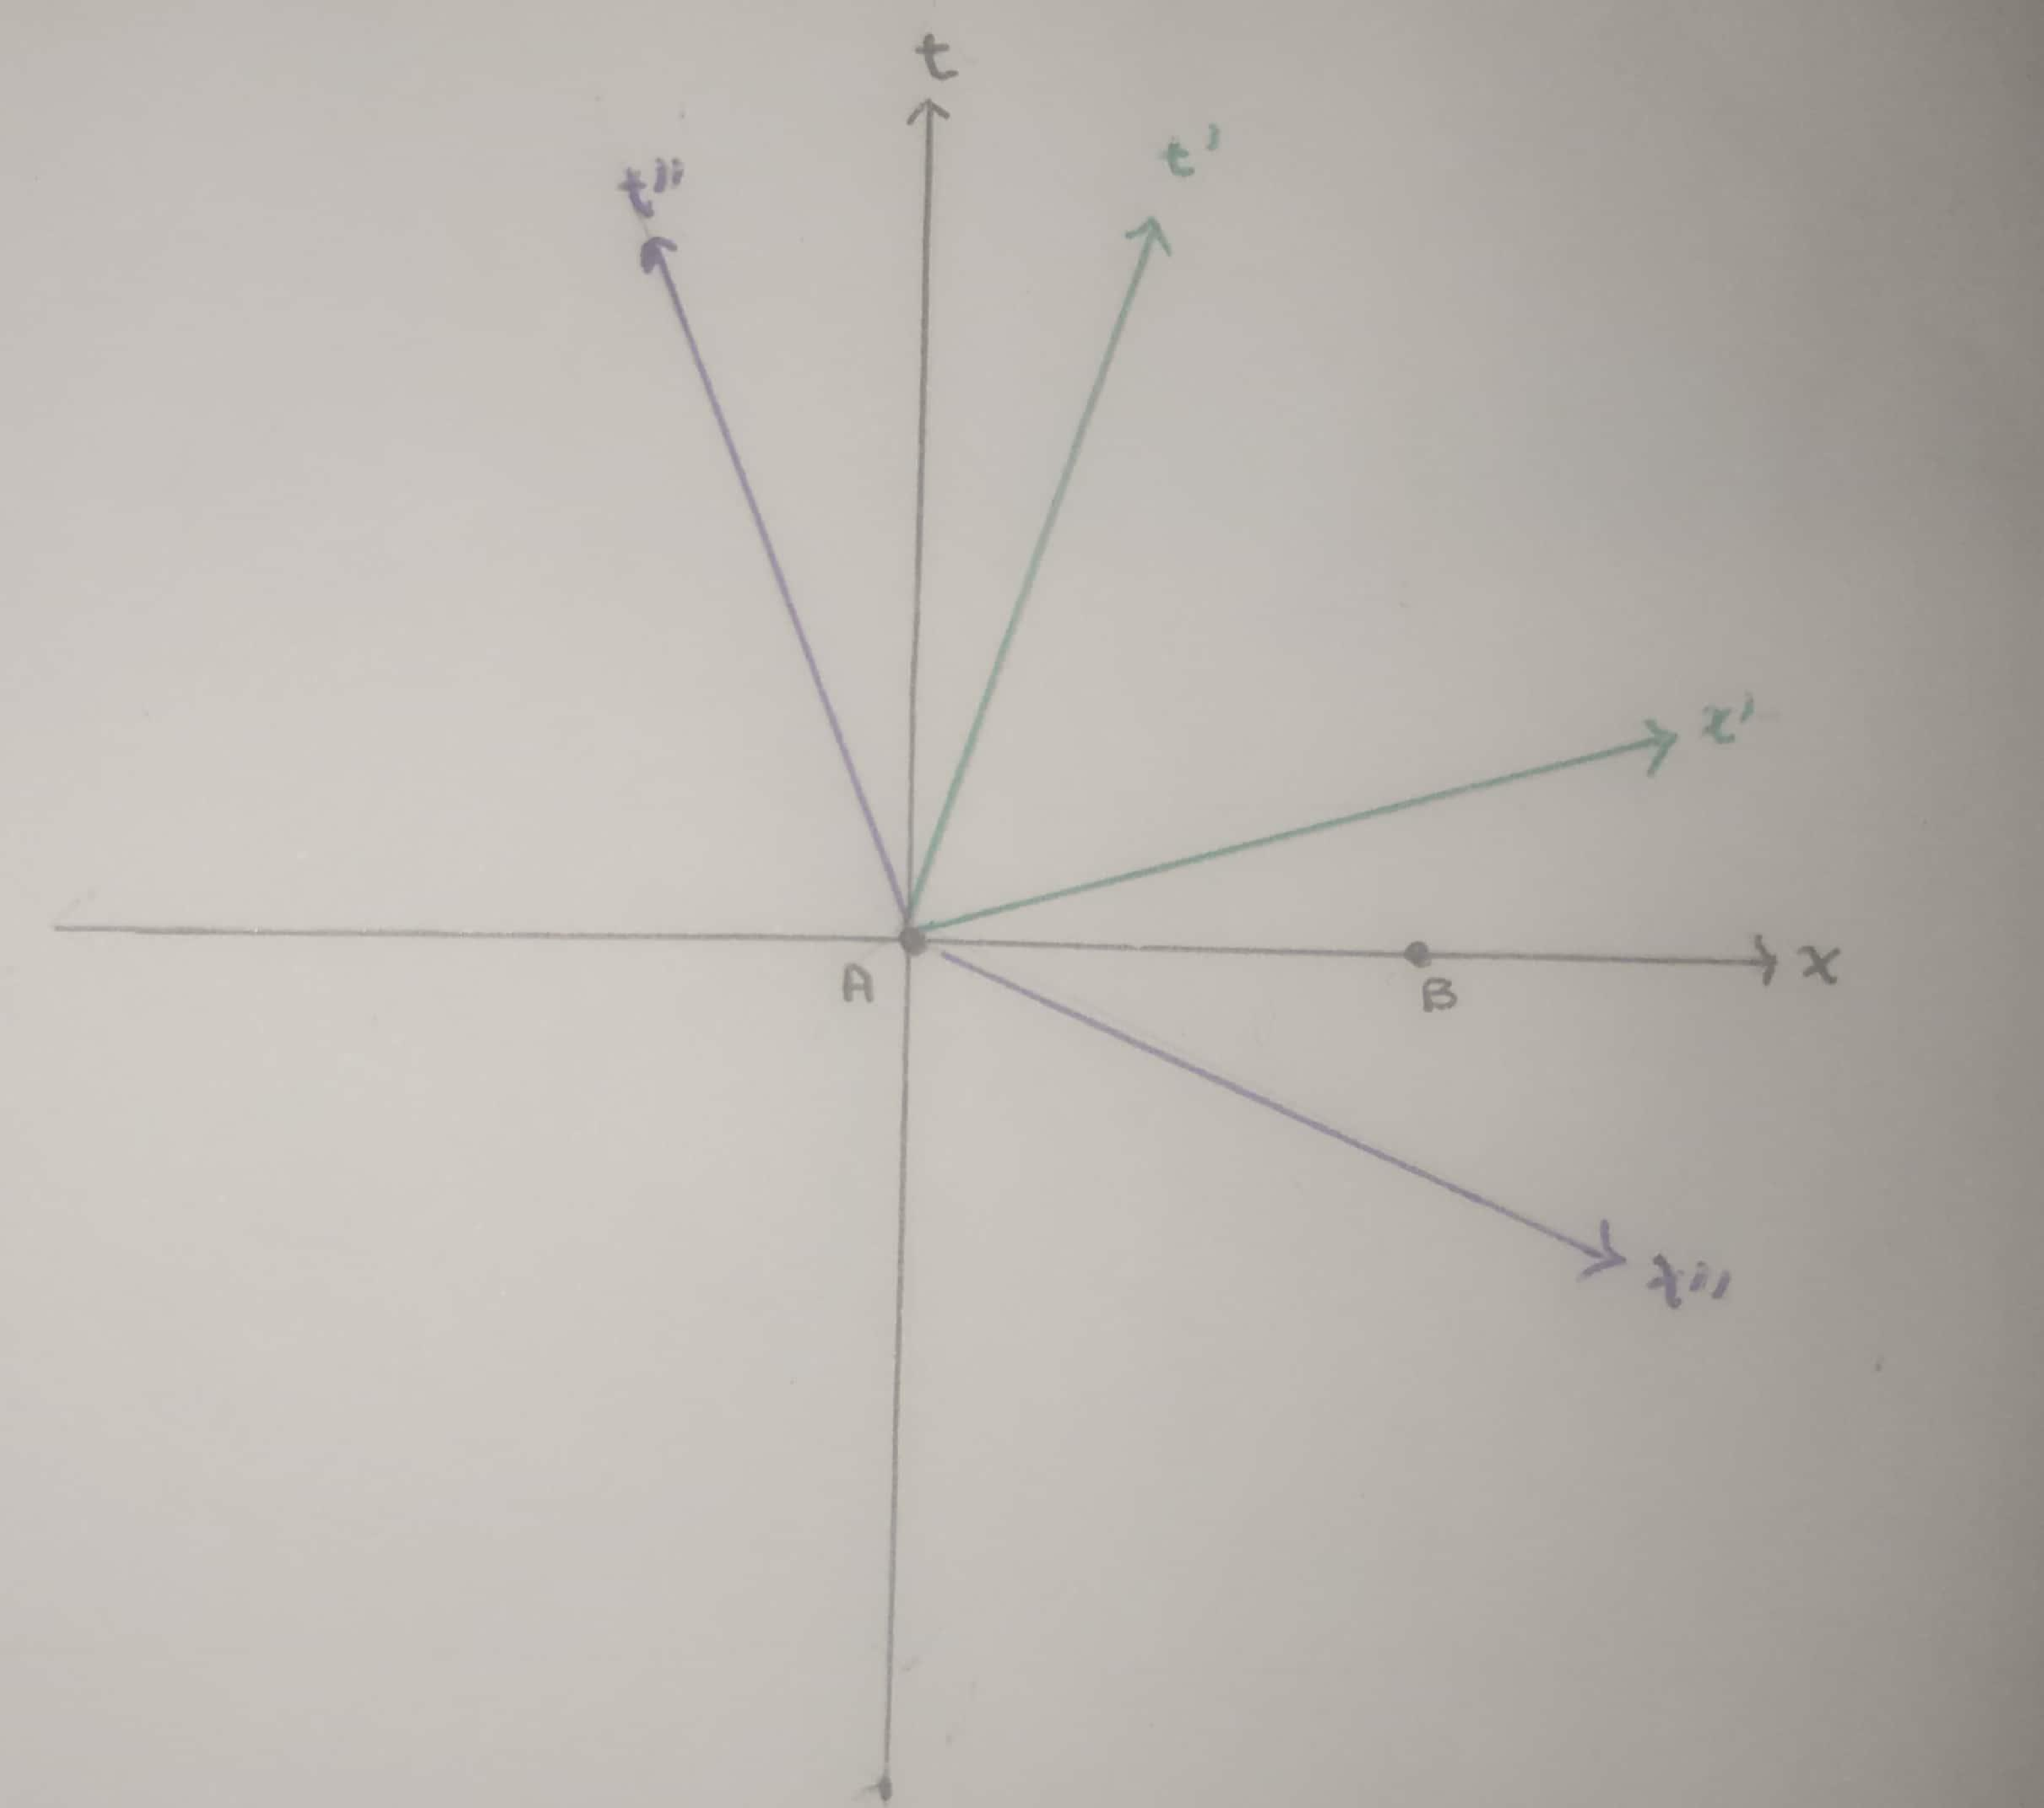
\includegraphics[scale = 0.15]{fig-2.1.pdf}
                \caption{Ejes coordenados de \(\primeobserver\) y \(\biprimeobserver\) en el diagrama de \(\observer\).}
                \label{fig:OprimeObiprimeInO}
            \end{figure}

            \pagebreak
            \item Elige algún evento \(B\) en el eje \(x\) (que no sea el origen) y márcalo en el diagrama. ¿Cuál es el tipo de separación que hay entre \(A\) y \(B\)? Recuerda que esta respuesta es independiente del sistema de referencia que use para hacer el cálculo.
            
            \inlinesol
            
            En la \cref{fig:ABEventsInO}, se muestran los conos de luz para los eventos \(A\) y \(B\), respectivamente. 

            \begin{figure}[htb]
                \centering
                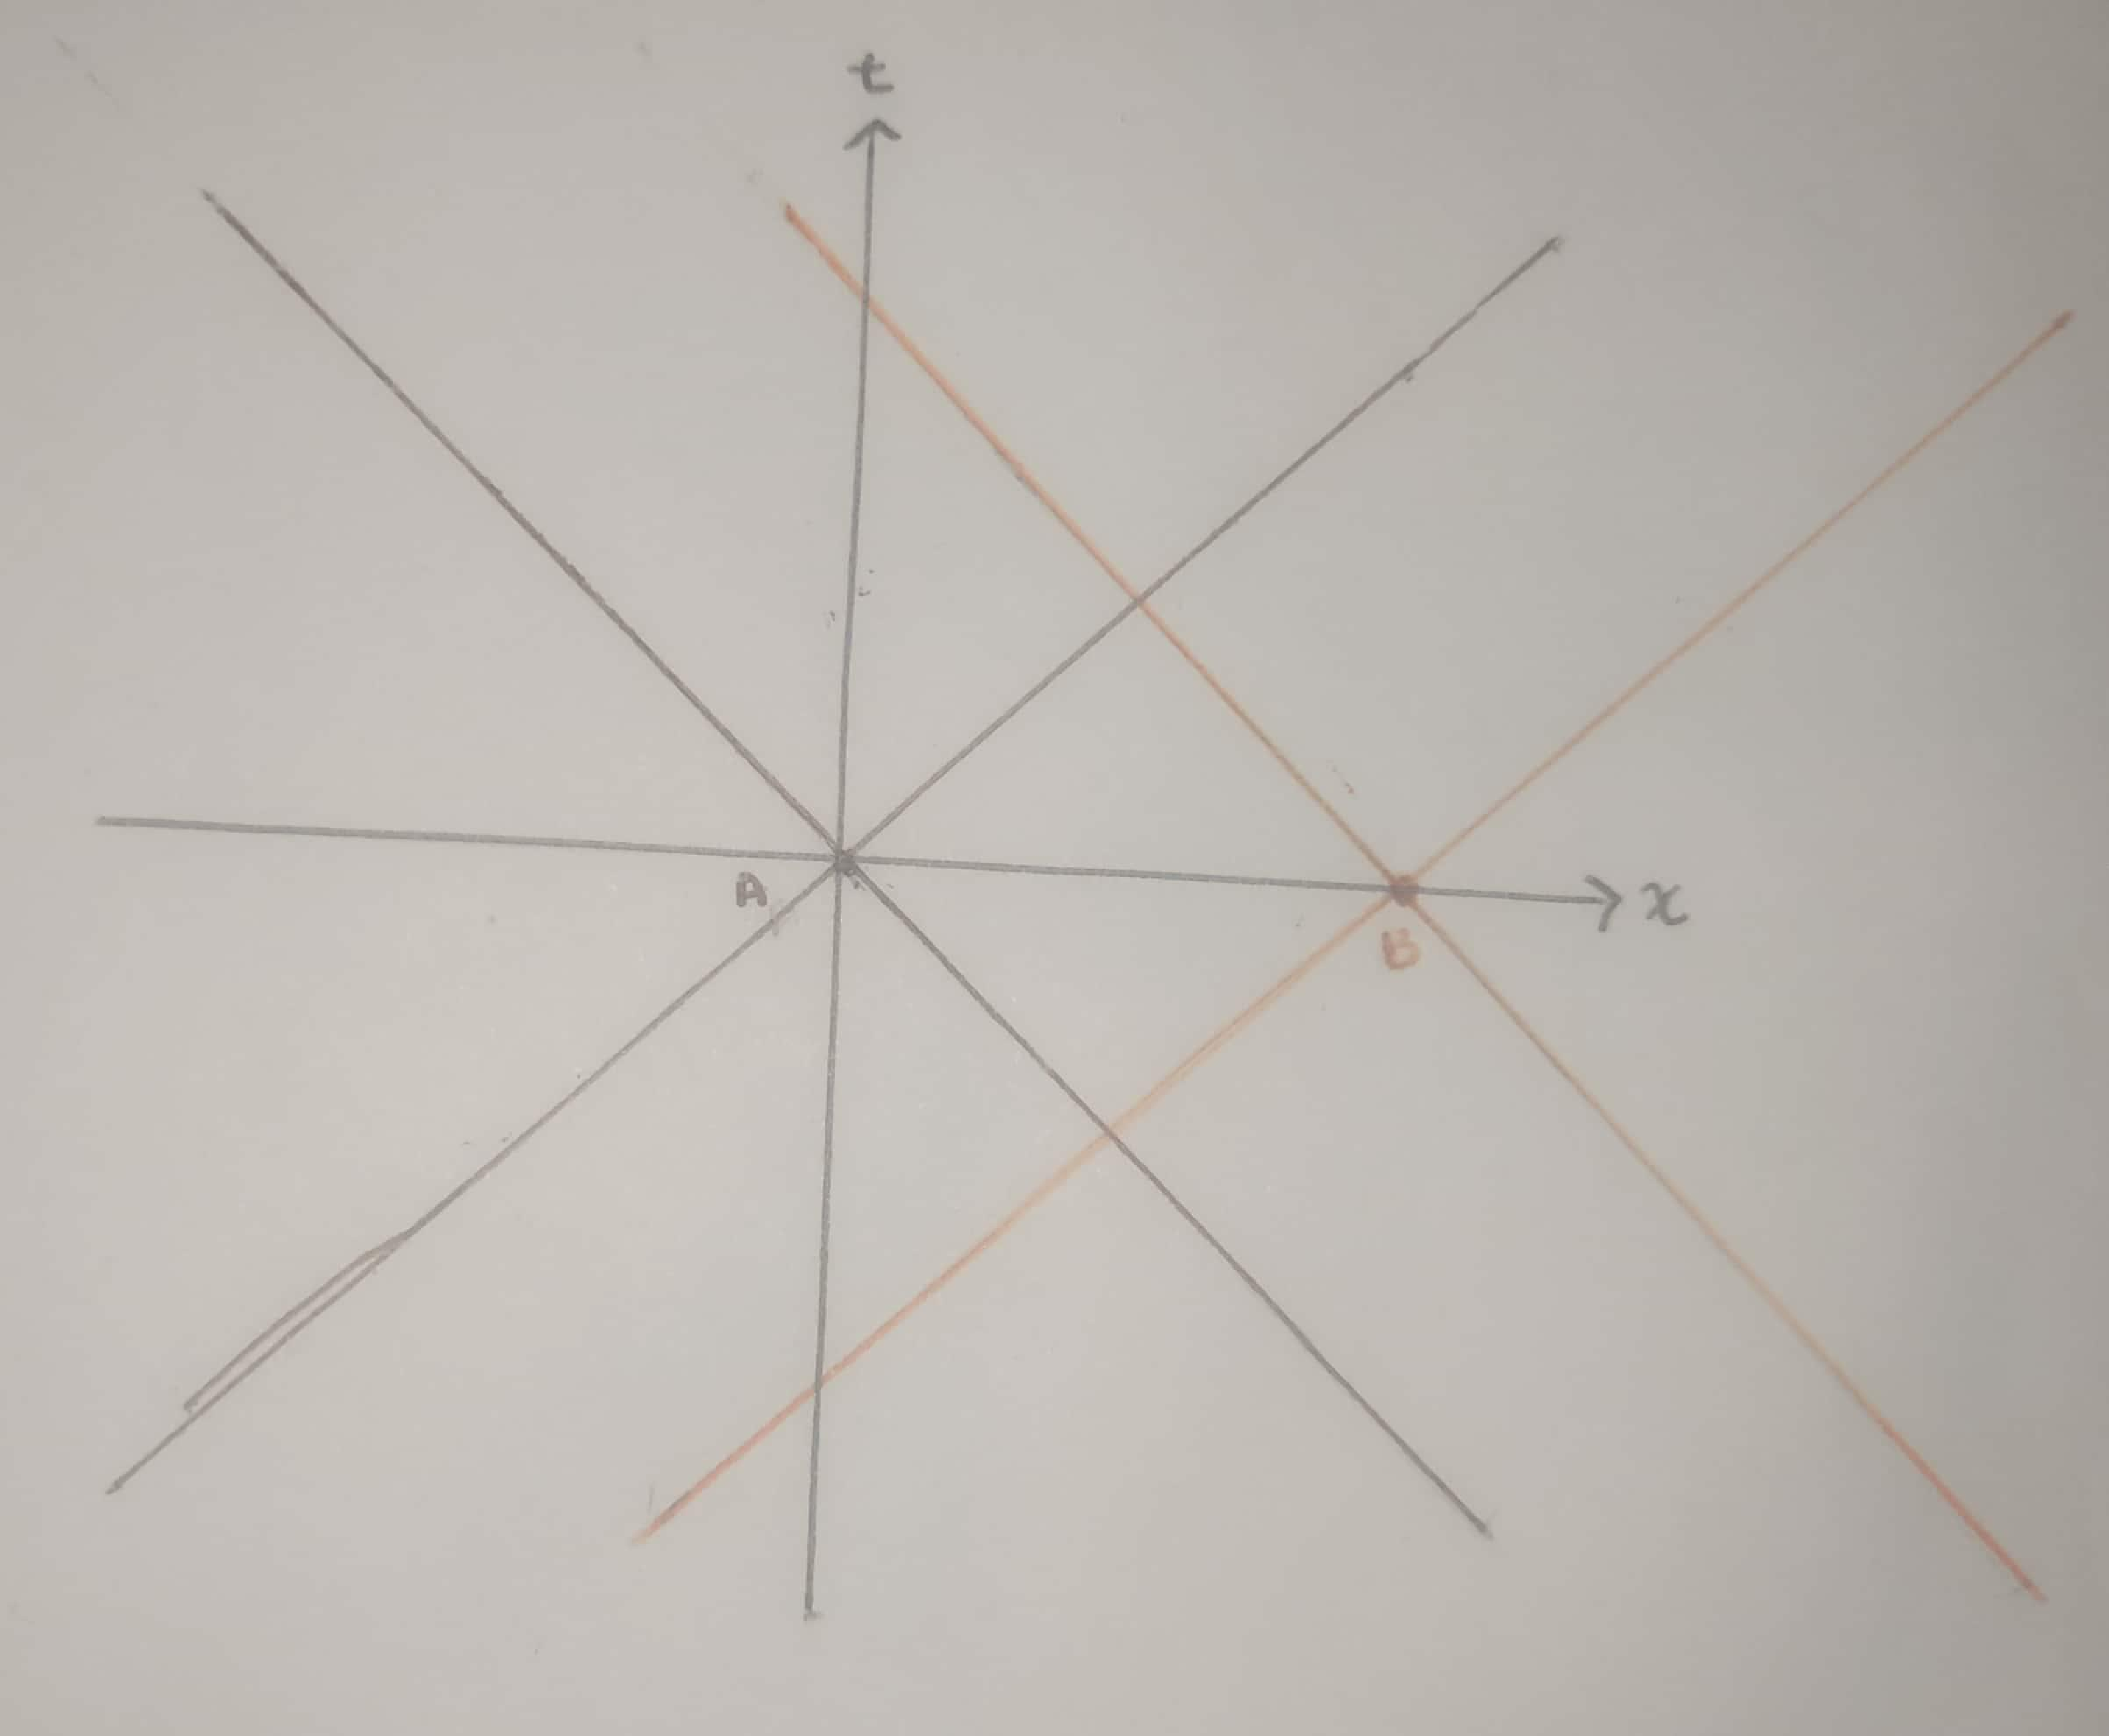
\includegraphics[scale = 0.15]{fig-2.2.pdf}
                \caption{Conos de luz de los eventos \(A\) y \(B\).}
                \label{fig:ABEventsInO}
            \end{figure}

            Notamos entonces que para el evento \(A\), \(B\) está fuera su cono de luz y, para \(B\), \(A\) está fuera de su cono de luz. Esto quiere decir que para el observador \(\observer\), la separación entre \(A\) y \(B\) es espacialoide, \textbf{i.e.}, \((\Delta s)^{2} > 0\).

            Analíticamente podemos determinar que la afirmación anterior es verdadera. Así,
            
            \begin{align*}
                (\Delta s)^{2} &= -(t_{B} - t_{A})^{2} + (x_{B} - x_{A})^{2},\\
                &= -(0 - 0)^{2} + (x_{B} - 0)^{2},\\
                (\Delta s)^{2} &= {x_{B}}^{2}. 
            \end{align*}

            En particular notamos que \(B\) es un evento diferente del origen, por lo que \(x_{B} \neq 0 \implies {x_{B}}^{2} > 0\). Por lo tanto,

            \begin{empheq}[box = \color{pinkwave}\fbox]{equation*}
                (\Delta s)^{2} > 0.
            \end{empheq}

            \item ¿Según \(\observer\) qué evento ocurre primero, \(A\) o \(B\)?
            
            \inlinesol

            Para \(\observer\) los eventos \(A\) y \(B\) son simultáneos, ya que ocurren al tiempo \(t = 0\).

            \item ¿Según \(\primeobserver\) qué evento ocurre primero, \(A\) o \(B\)? Pinta la línea de los eventos que son simultáneos a \(B\) según \(\primeobserver\).
            
            \inlinesol

            Para determinar cuál de los eventos ocurre primero, dibujamos los ejes de \(\observer\) en el diagrama de \(\primeobserver\), así como los eventos.

            De tal manera que observamos que para \(\primeobserver\), el evento \(B\) ocurre primero. Y, además, los eventos simultáneos a \(B\) son aquellos que ocurren al tiempo \(t^{\prime} = {t_{B}}^{\prime}\) (véase \cref{fig:ABInOPrime}).

            \begin{figure}[htb]
                \centering
                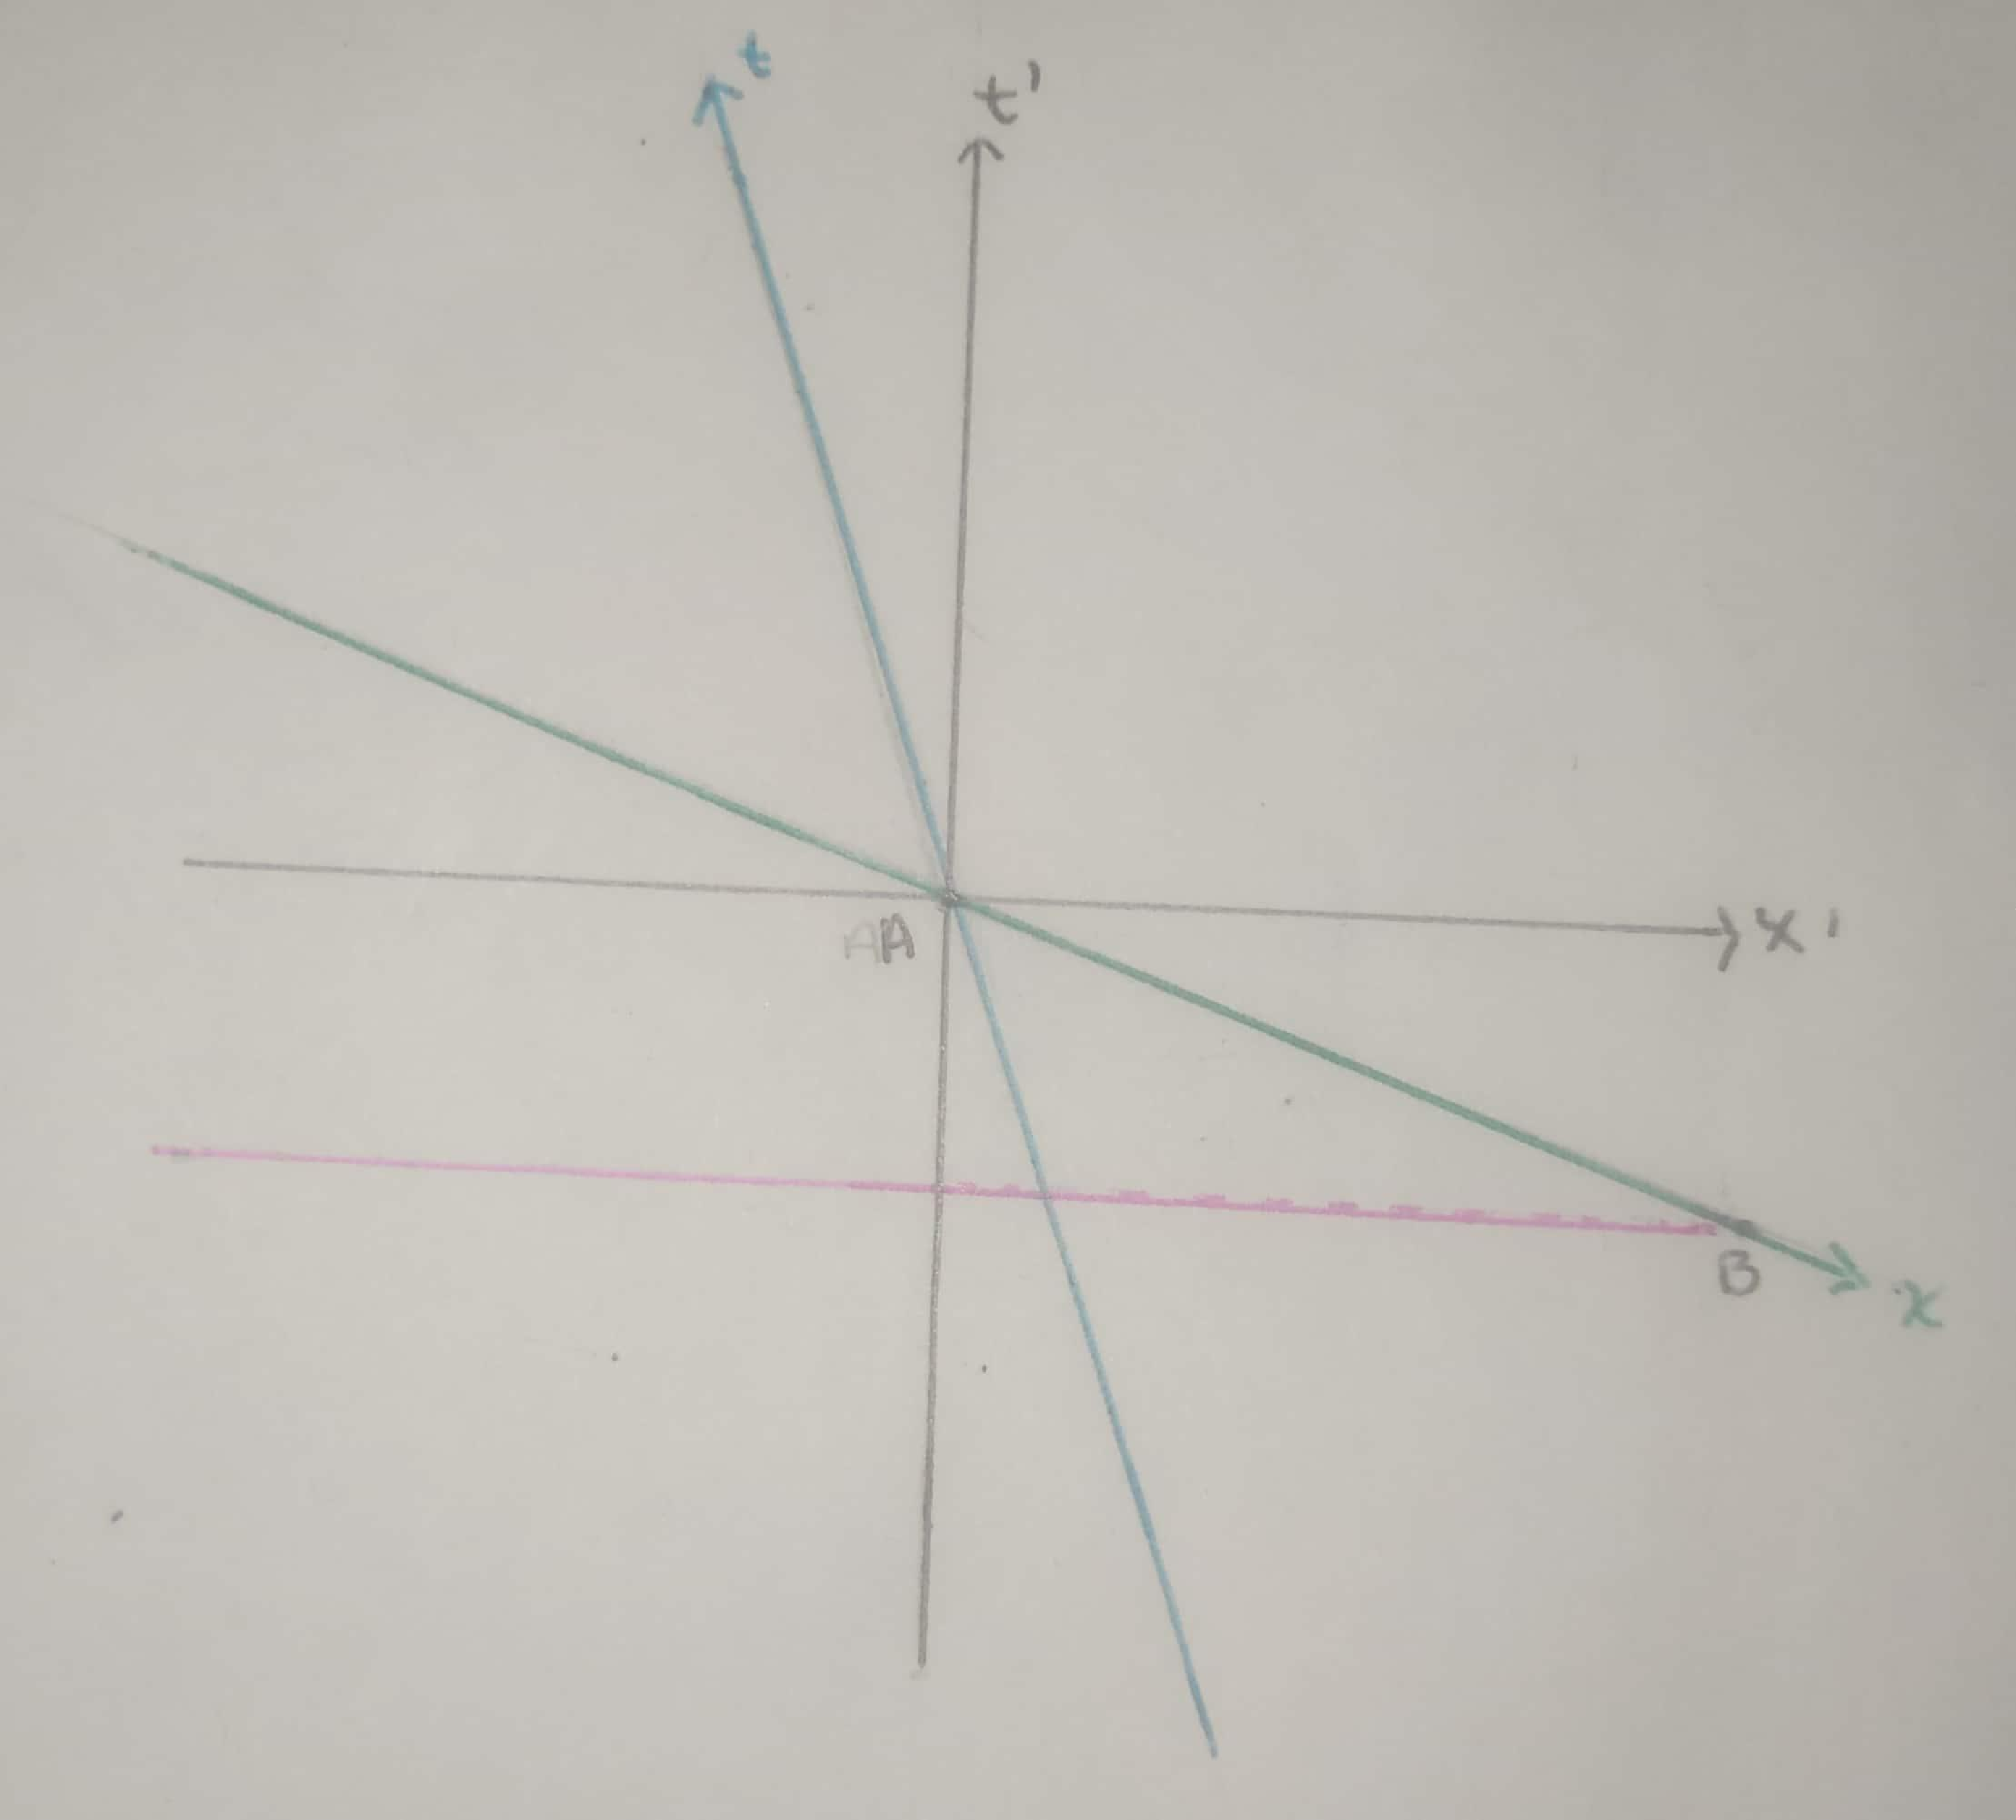
\includegraphics[scale = 0.15]{fig-2.3.pdf}
                \caption{Eventos \(A\) y \(B\) dibujados en el diagrama de \(\primeobserver\).}
                \label{fig:ABInOPrime}
            \end{figure}

            \pagebreak
            \item ¿Según \(\biprimeobserver\) qué evento ocurre primero, \(A\) o \(B\)? Pinta la línea de los eventos que son simultáneos a \(B\) según \(\biprimeobserver\).
            
            \inlinesol

            Los ejes de \(\primeobserver\) dibujados en el diagrama de \(\biprimeobserver\) queda igual que los ejes de \(\primeobserver\) en el diagrama de \(\observer\). Esto se debe a que \(\biprimeobserver\) observa que \(\observer\) se aleja con velocidad \(v > 0\) respecto a éste (véase \cref{fig:OInOPrimePrime}).
            
            De esta manera, notamos que para \(\biprimeobserver\) el evento \(A\) ocurre primero. Y los eventos simultáneos a \(B\) ocurren a \(t^{\prime\prime} = {t_{B}}^{\prime\prime}\).

            \begin{figure}[htb]
                \centering
                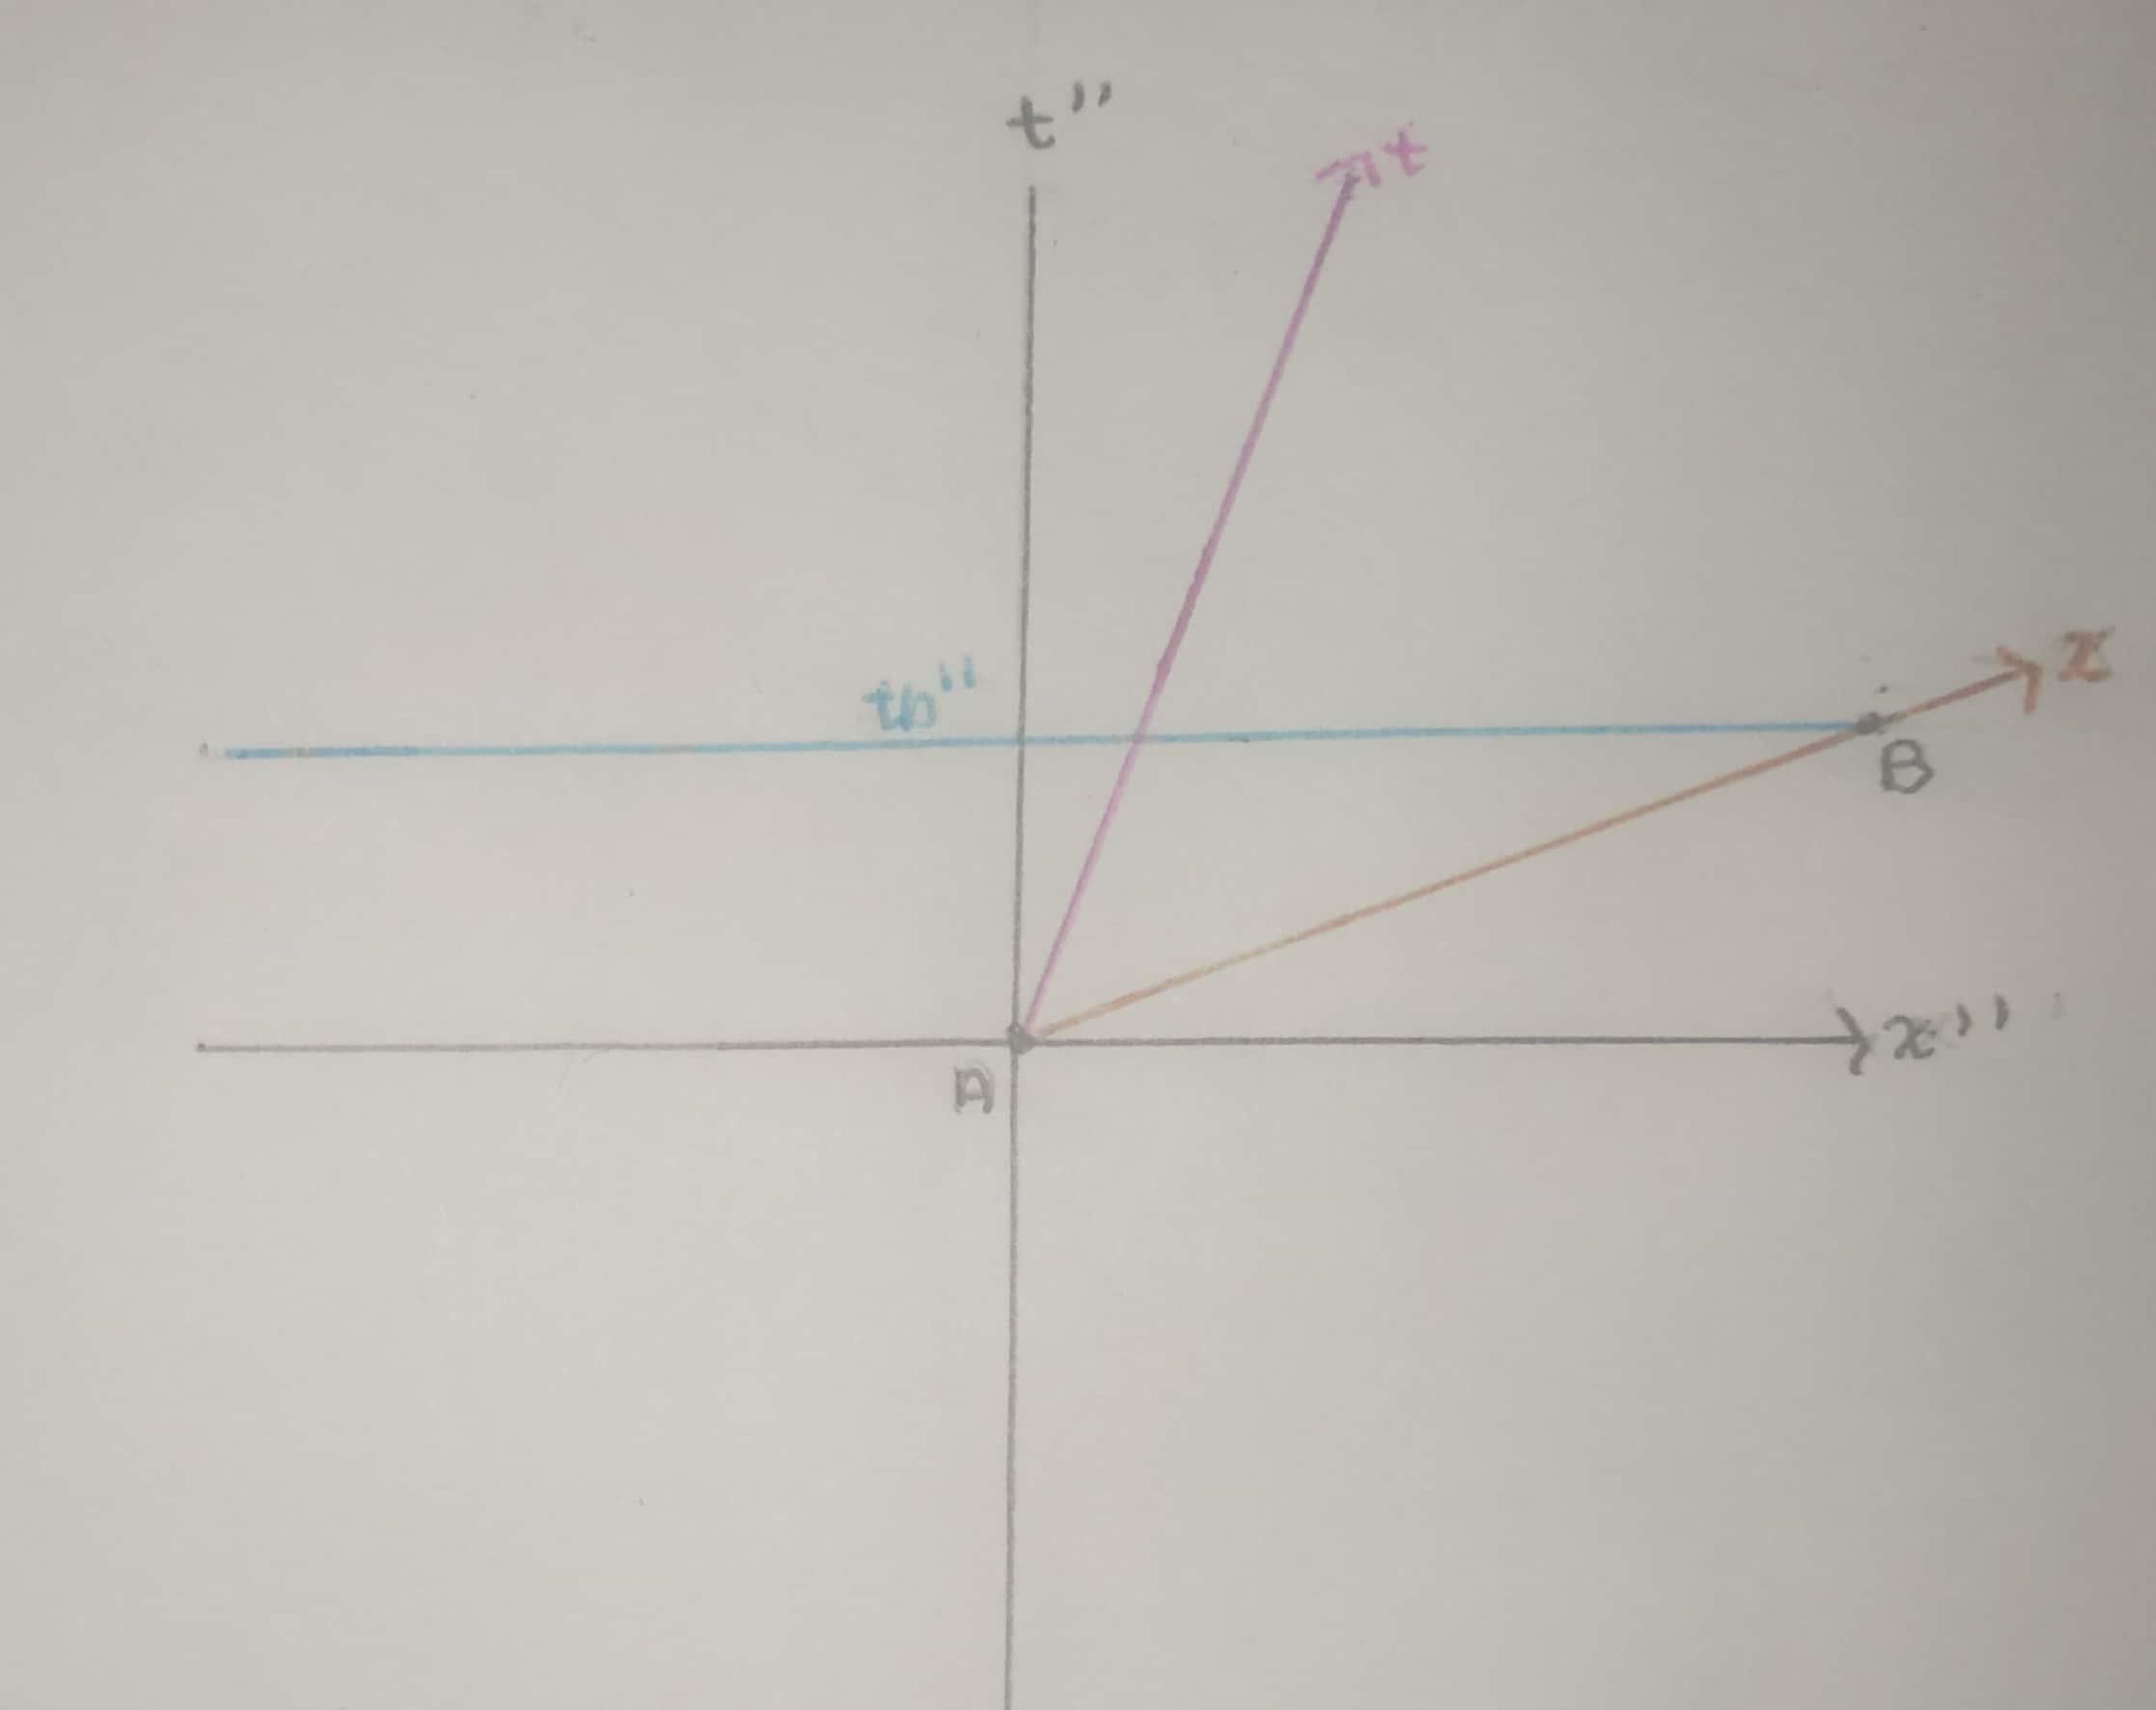
\includegraphics[scale = 0.15]{fig-2.4.pdf}
                \caption{Ejes de \(\observer\) dibujados en el diagrama de \(\biprimeobserver\), así como la línea de los eventos simultáneos al evento \(B\).}
                \label{fig:OInOPrimePrime}
            \end{figure}

            \pagebreak
            \item Elige ahora un evento \(C\) en el eje \(t\) (que no sea el origen) y márcalo en el diagrama. ¿Cuál es el tipo de separación que hay entre \(A\) y \(C\)? Recuerda que esta respuesta es independiente del sistema de referencia que uses para hacer el cálculo.
            
            \inlinesol

            Dibujamos un punto \(C\) (véase \cref{fig:ABIntervalInO}), tal que \(x = 0\), \textbf{i.e.}, \((c, 0)\), con \(c \neq 0\). Además, dibujamos el cono de luz correspondiente a cada evento, tenemos que la separación entre estos es de tipo \setulcolor{pinkwave}\ul{temporaloide}.

            Analíticamente podemos comprobar esta afirmación, tal que,
            
            \begin{align*}
                (\Delta s)^{2} &= -(t_{C} - t_{A})^{2} + (x_{C} - x_{A})^{2},\\
                &= -(t_{C} - 0)^{2} + (0 - 0)^{2},\\
                &= -(t_{C})^{2}.
            \end{align*}

            \begin{figure}[htb]
                \centering
                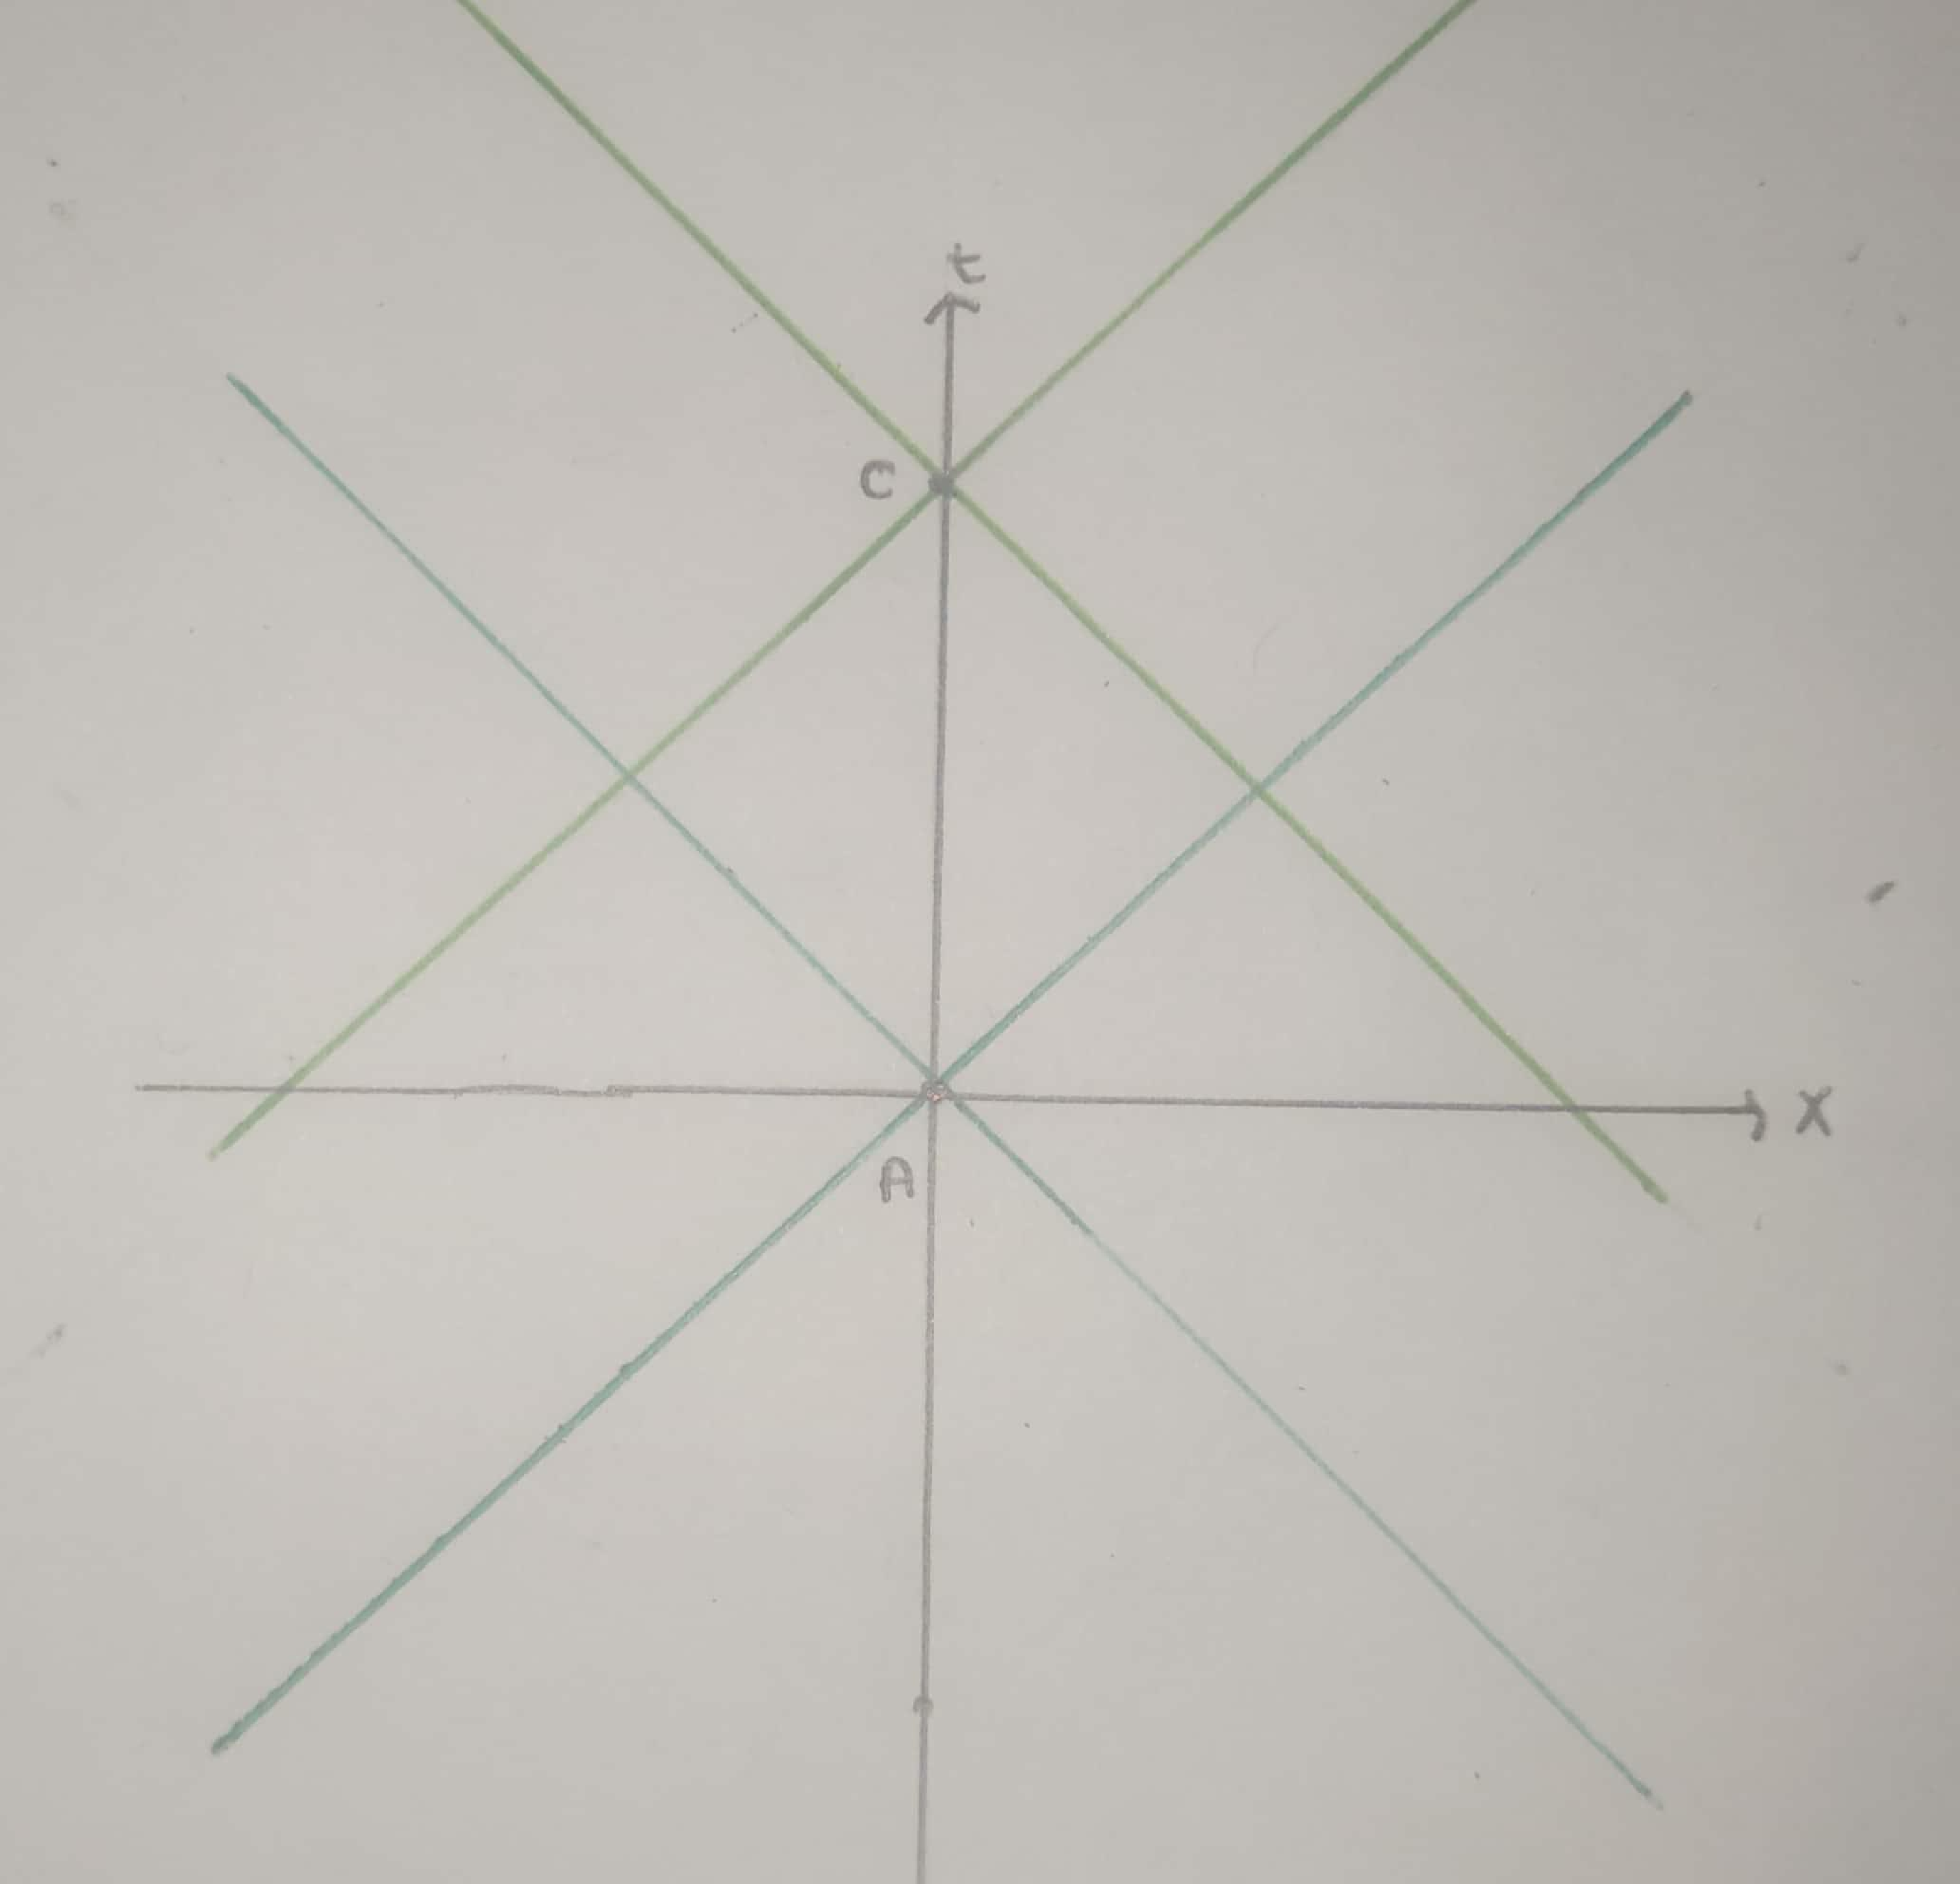
\includegraphics[scale = 0.15]{fig-2.5.pdf}
                \caption{Conos de luz correspondientes a los eventos \(A\) y \(B\) para determinar el tipo de separación que hay entre estos.}
                \label{fig:ABIntervalInO}
            \end{figure}

            Notamos entonces que sin importar que el evento \(C\) suceda antes o después del evento \(A\), su intervalo siempre será \((\Delta s)^{2} < 0\), lo cual nos permite, una vez más, concluir que la separación entre los eventos es temporaloide. 

            \item ¿Según \(\observer\) qué evento ocurre primero, \(A\) o \(C\)?
            
            Por como dibujamos el evento \(C\) en la \cref{fig:ABIntervalInO}, tenemos que para \(\observer\) el evento \(A\) ocurre primero.

            \item ¿Según \(\primeobserver\) qué evento ocurre primero, \(A\) o \(C\)? Pinta la línea de los eventos que son simultáneos a \(C\) según \(\primeobserver\).
            
            \inlinesol

            Ahora queremos determinar cuál de los eventos del inciso e) ocurre primero para \(\primeobserver\). Dibujamos el diagrama de espacio-tiempo de la \cref{fig:ABInOPrime}, agregando el evento \(C\).

            Observamos entonces que para \(\primeobserver\) el evento que ocurre primero es \(A\) y, además, los eventos simultáneos a \(C\) son aquellos que ocurren al tiempo \(t^{\prime} = {t_{C}}^{\prime}\) (véase \cref{fig:ACInOPrime}).

            \begin{figure}[htb]
                \centering
                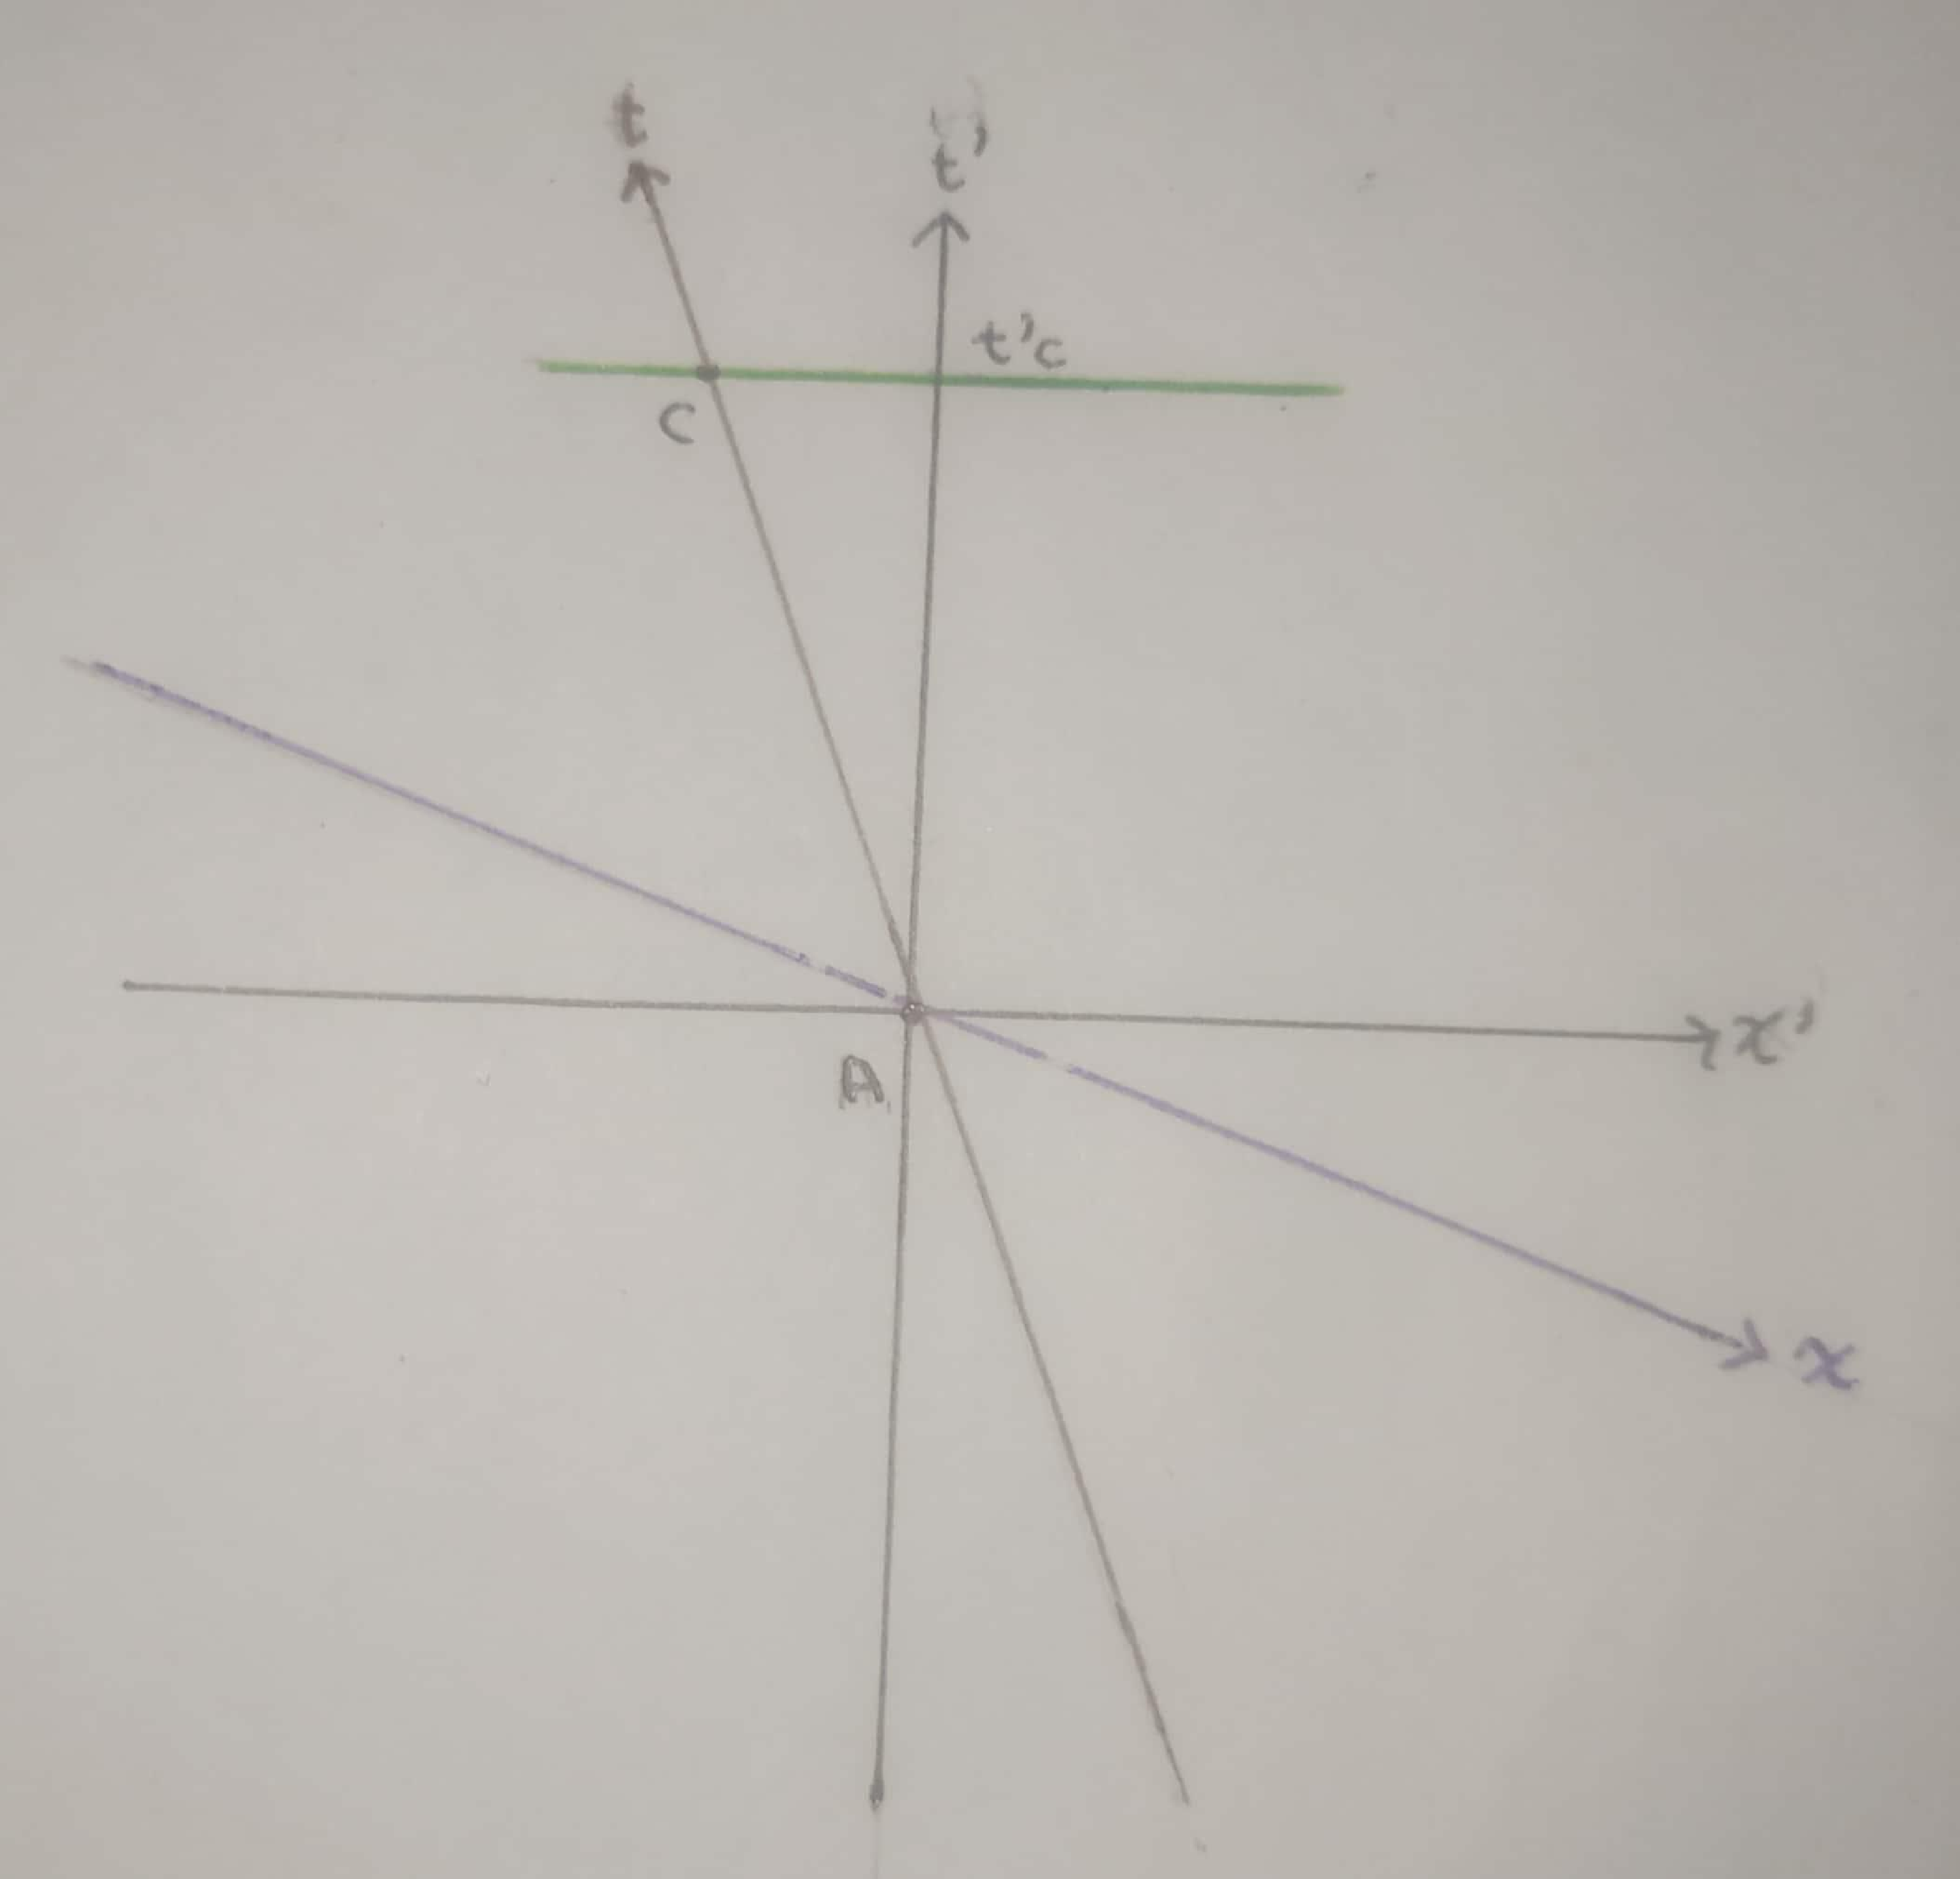
\includegraphics[scale = 0.15]{fig-2.6.pdf}
                \caption{Eventos \(A\) y \(C\) dibujados en el diagrama de \(\primeobserver\), así como la línea de los eventos simultáneos a \(C\).}
                \label{fig:ACInOPrime}
            \end{figure}

            \pagebreak
            \item ¿Según \(\biprimeobserver\) qué evento ocurre primero, \(A\) o \(C\)? Pinta la línea de los eventos que son simultáneos a \(C\) según \(\biprimeobserver\).
            
            \inlinesol

            Replicando el diagrama de la \cref{fig:OInOPrimePrime} agregando el evento \(C\), tenemos que directamente podemos determinar que el evento \(A\) ocurre primero para el observador \(\biprimeobserver\) y, además, los eventos simultáneos a \(C\) son aquellos que ocurren a \(t^{\prime\prime} = {t_{C}}^{\prime\prime}\) (véase \cref{fig:ACInOPrimePrime}).

            \begin{figure}[htb]
                \centering
                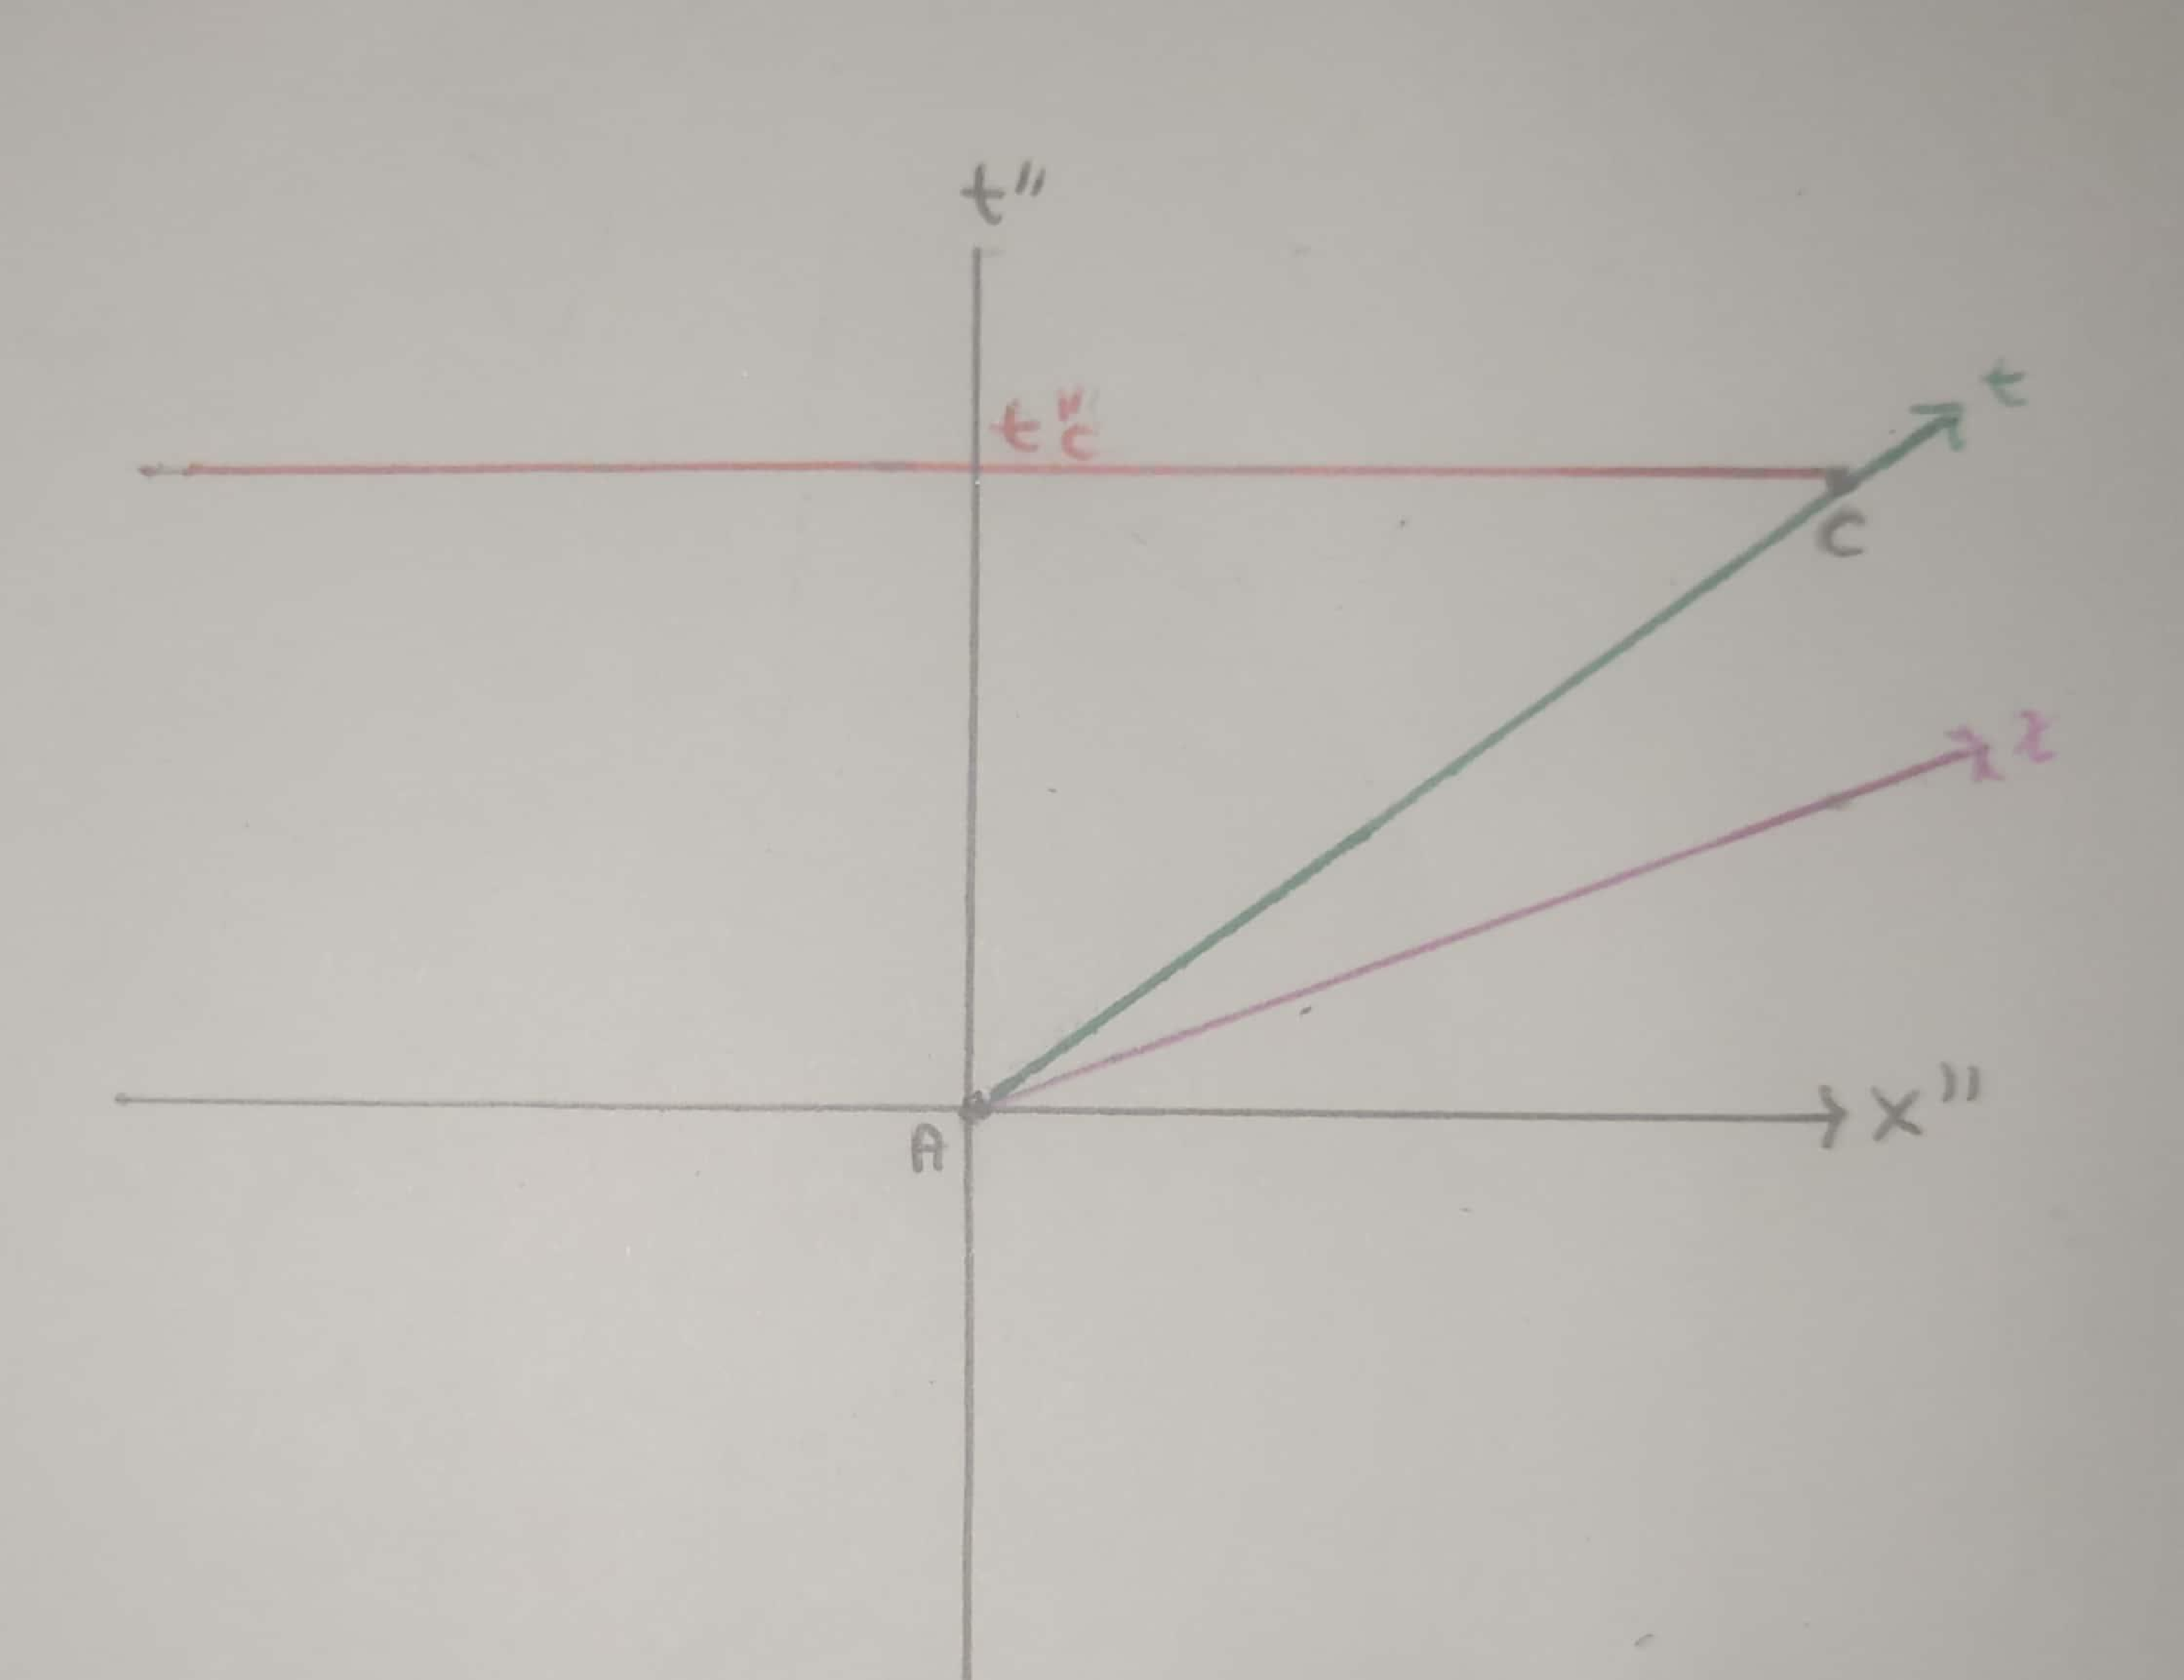
\includegraphics[scale = 0.15]{fig-2.7.pdf}
                \caption{Eventos \(A\) y \(C\) dibujados en el diagrama de \(\biprimeobserver\), así como la línea de los eventos simultáneos a \(C\).}
                \label{fig:ACInOPrimePrime}
            \end{figure}
        \end{enumerate}
    \end{exercise}

    \pagebreak
    \begin{exercise}
        Es útil aprender a visualizar el intervalo entre dos eventos en los diagramas de espacio-tiempo, similar a como sabemos visualizar la distancia entre dos puntos en el espacio Euclidiano. Considera así un espacio-tiempo 1+1-dimensional y dos observadores inerciales \(\observer\) y \(\primeobserver\) en éste, tales que \(\primeobserver\) se mueve con velocidad \(v > 0\) respecto a \(\observer\). El origen de ambos está colocado en el origen.

        \begin{enumerate}[label = \alph*)]
            \item Localiza en el diagrama de \(\observer\) al evento \(B\) de coordenadas \((b, 0)\) con \(b > 0\).
            
            \inlinesol

            El punto \(B\) se localiza en la parte positiva del eje \(t\) (véase la \cref{fig:Bequalsb0InO}).

            \begin{figure}[htb]
                \centering
                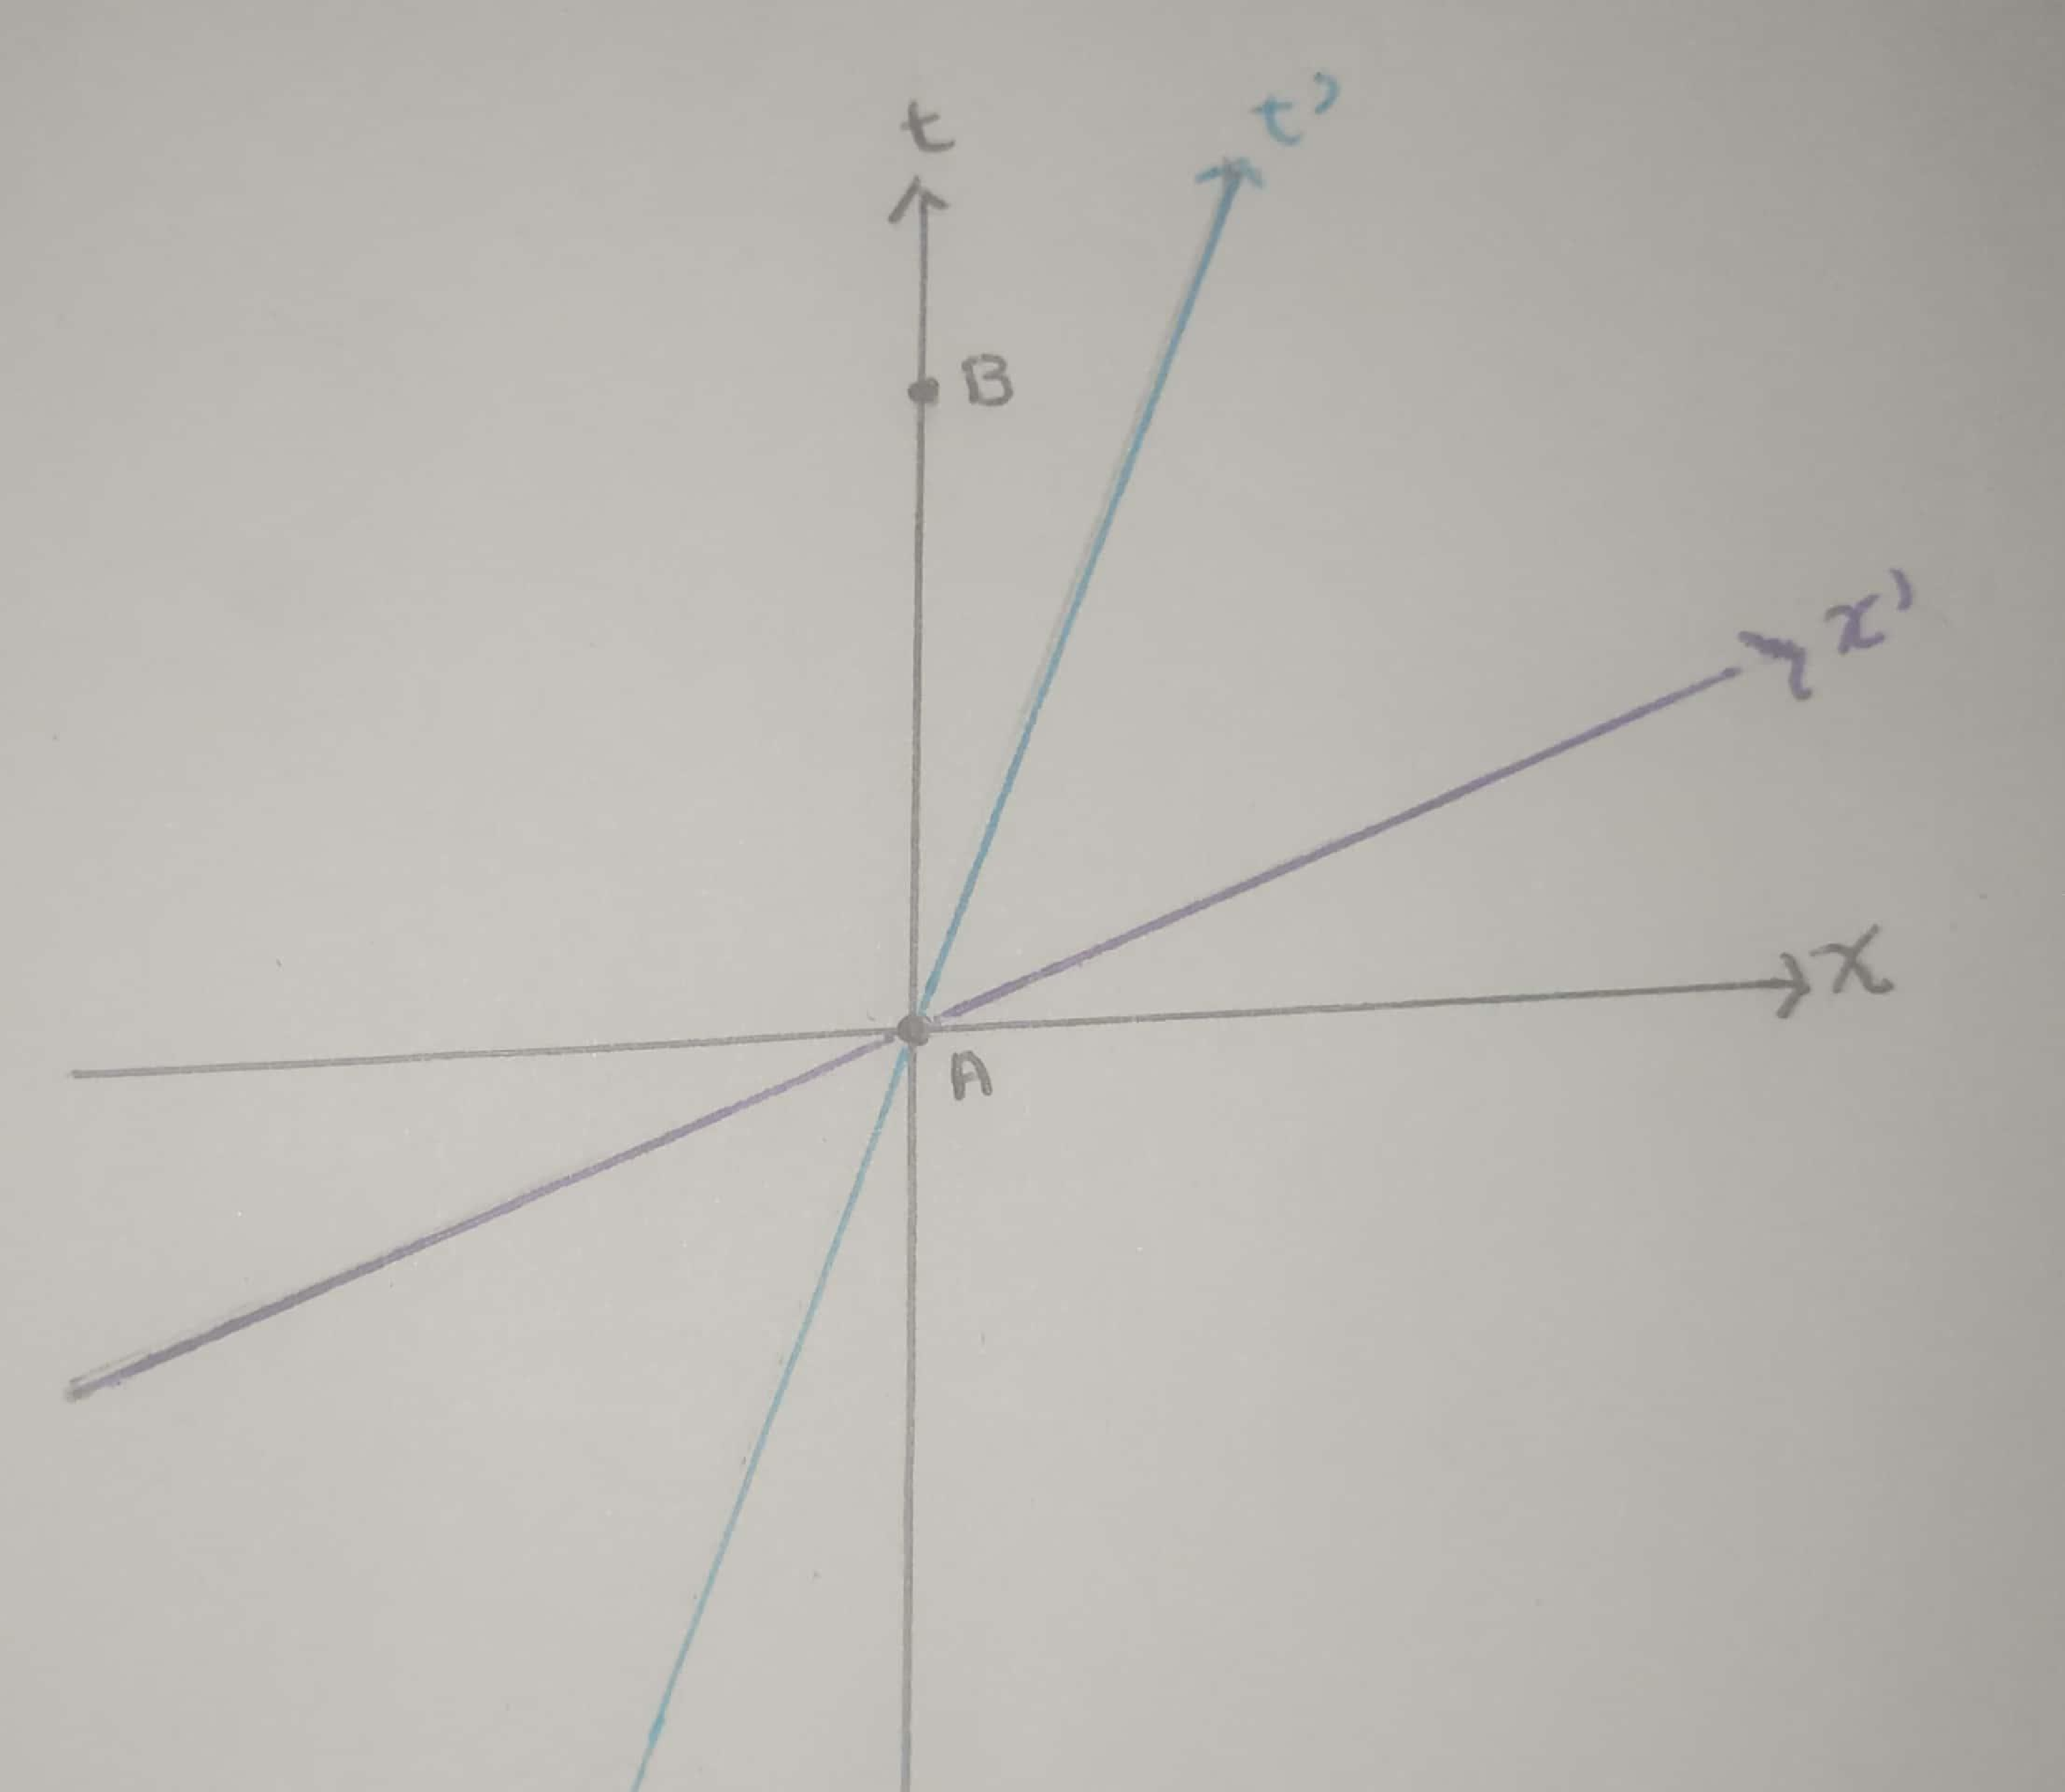
\includegraphics[scale = 0.15]{fig-2.8.pdf}
                \caption{Evento \(B = (b, 0)\) dibujado en el diagrama de espacio-tiempo de \(\observer\).}
                \label{fig:Bequalsb0InO}
            \end{figure}

            \item Calcula el intervalo \((\Delta s_{AB})^{2}\) entre \(A\) y \(B\). ¿Qué tipo de separación hay entre estos eventos?
            
            Calculamos el intervalo entre los eventos \(A\) y \(B\), tal que,

            \begin{align}
                (\Delta s_{AB})^{2} &= -(t_{B} - t_{A})^{2} + (x_{B} - x_{A})^{2},\nonumber\\
                &= -(b - 0)^{2} + (0 - 0)^{2},\nonumber\\
                \Acolorboxed{(\Delta s_{AB})^{2} &= -b^{2}.}
                \label{eq:IntervalAB}
            \end{align}

            \pagebreak
            De la \cref{eq:IntervalAB}, tenemos que

            \begin{equation*}
                (\Delta s_{AB})^{2} < 0
            \end{equation*}

            Por lo tanto, la separación entre los eventos es de tipo \setulcolor{pinkwave}\ul{temporaloide}.

            \item Escribe la ecuación del lugar geométrico de todos los eventos \(C\) tales que \((\Delta s_{AC})^{2} = (\Delta s_{AB})^{2}\), es decir, de todos los eventos que equidistan espacio-temporalmente de \(A\). Pinta este lugar geométrico en el diagrama de \(\observer\) (ambas ramas).
            
            \inlinesol

            Sea \(C\) un evento distinto del origen, tal que \((\Delta s_{AB})^{2} = (\Delta s_{AC})^{2}\). Sustituyendo la \cref{eq:IntervalAB} en la aseveración anterior,

            \begin{align*}
                -b^{2} &= -(t_{C} - t_{A})^{2} + (x_{C} - x_{A})^{2},\nonumber\\
                &= -(t_{C} - 0)^{2} + (x_{C} - 0)^{2},\nonumber\\
                \Aboxed{-b^{2} &= -{t_{C}}^{2} + {x_{C}}^{2}.}
            \end{align*}

            Reescribiendo la expresión anterior,

            \begin{empheq}[box = \color{pinkwave}\fbox]{equation}
                -\dfrac{{x_{C}}^{2}}{b^{2}} + \dfrac{{t_{C}}^{2}}{b^{2}} = 1.
                \label{eq:hyperbole}
            \end{empheq}

            El lugar geométrico de todos los puntos que equidistan al evento \(A\) se muestra en la \cref{fig:hyperbole}.
            
            \begin{figure}[htb]
                \centering
                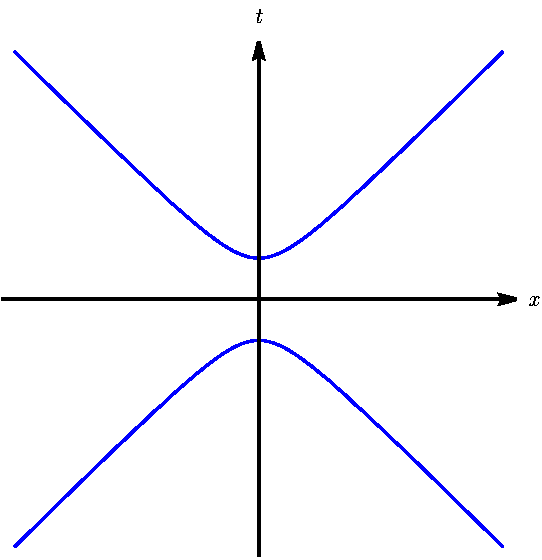
\includegraphics{hyperbole.pdf}
                \caption{Lugar geométrico de los puntos equidistantes a \(B\), dado por \(-\frac{x^{2}}{b^{2}} + \frac{t^{2}}{b^{2}} = 1\).}
                \label{fig:hyperbole}
            \end{figure}

            \item Pinta los ejes de \(\primeobserver\) em el diagrama de \(\observer\). ¿El lugar geométrico que encontraste en el inciso c) intersecta con el eje \(t^{\prime}\)? ¿En qué eventos? Márcalos en el diagrama.
            
            \inlinesol
            
            Para encontrar en que punto se intersectan la \cref{eq:hyperbole} y el eje \(t^{\prime}\) debemos igualar las expresiones, pero primero debemos resolver la \cref{eq:hyperbole} para \(x\), tal que,

            \begin{equation}
                \boxed{x = \sqrt{t^{2} - b^{2}}.}
                \label{eq:hyperboleBranches}
            \end{equation}

            Igualando la \cref{eq:hyperboleBranches} y \(x = vt\) (ecuación de \(t^{\prime}\)).

            \begin{align}
                vt &= \sqrt{t^{2} - b^{2}},\nonumber\\
                v^{2}t^{2} &= t^{2} - b^{2},\nonumber\\
                \Acolorboxed{t &= \pm \dfrac{b}{\sqrt{1 - v^{2}}}.}
                \label{eq:TValuesIntersection}
            \end{align}

            \pagebreak
            Sustituyendo la \cref{eq:TValuesIntersection} en \(x = vt\),

            \begin{empheq}[box = \color{pinkwave}\fbox]{equation}
                \begin{aligned}
                    x_{1} &= \dfrac{vb}{\sqrt{1 - v^{2}}},\\
                    x_{2} &= \dfrac{-vb}{\sqrt{1 - v^{2}}}.
                \end{aligned}
                \label{eq:XValuesIntersection}
            \end{empheq}

            Así, de las \cref{eq:TValuesIntersection,eq:XValuesIntersection}, los puntos de intersección son:

            \begin{empheq}[box = \color{pinkwave}\fbox]{align}
                \zeta &= \left(\dfrac{b}{\sqrt{1 - v^{2}}}, \dfrac{-vb}{\sqrt{1 - v^{2}}}\right),\label{eq:EventD}\\
                \zeta^{\prime} &= \left(\dfrac{-b}{\sqrt{1 - v^{2}}}, \dfrac{-vb}{\sqrt{1 - v^{2}}}\right)\nonumber.
            \end{empheq}

            En la \cref{fig:HyperboleTPrimeIntersection} se muestra los eventos en los que se intersectan las \cref{eq:hyperbole} y el eje \(t^{\prime}\).

            \begin{figure}[htb]
                \centering
                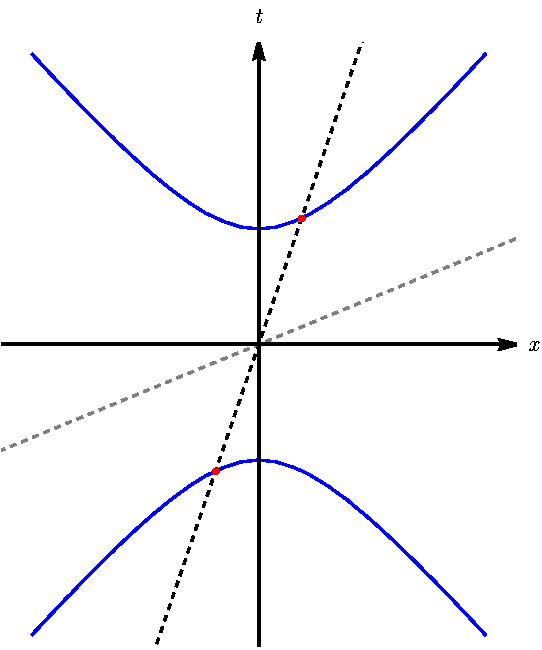
\includegraphics{intersection.pdf}
                \caption{Intersección del lugar geométrico de los eventos equidistantes a \(A\) y el eje \(t^{\prime}\), donde los ejes (en sentido de las manecillas del reloj) son \(t^{\prime}\) y \(x^{\prime}\).}
                \label{fig:HyperboleTPrimeIntersection}
            \end{figure}

            \pagebreak
            \item Denota a uno de los eventos que encontraste en d) como D. ¿Cuánto vale el intervalo \((\Delta s^{\prime}_{AD})^{2}\) entre \(D\) y \(A\) según \(\primeobserver\)? Recuerda: el intervalo es invariante.
            
            \inlinesol
            
            Ahora calculamos el intervalo entre los eventos \(D\) (\cref{eq:EventD}) y \(A\).

            \begin{align}
                (\Delta {s_{AD}}^{\prime})^{2} &= -\left(\dfrac{b}{\sqrt{1 - v^{2}}} - 0\right)^{2} + \left(\dfrac{-vb}{\sqrt{1 - v^{2}}} - 0\right)^{2},\nonumber\\
                &= -\dfrac{b^{2}}{1 - v^{2}} + \dfrac{v^{2}b^{2}}{1 - v^{2}},\nonumber\\
                &= \dfrac{-b^{2}}{1 - v^{2}}(1 - v^{2}),\nonumber\\
                \Acolorboxed{(\Delta {s_{AD}}^{\prime})^{2} &= -b^{2}.}\label{eq:ADInterval}
            \end{align}

            Notamos entonces de las \cref{eq:IntervalAB,eq:ADInterval},

            \begin{equation*}
                \boxed{(\Delta s_{AB})^{2} = (\Delta {s_{AD}}^{\prime})^{2}.}
            \end{equation*}

            \item Usa tu resultado de e) para escribir las coordenadas del evento \(D\) en el sistema \(\primeobserver\). Lo que acabas de hacer es escalar los ejes, es decir, has determinado lo que cada observador llama \(b\) metros.

            \inlinesol
            
            Puesto que el evento \(D\) se encuentra en el eje \(t^{\prime}\), lo único que necesitamos para escribirlo en coordenadas del sistema \(\primeobserver\) es hacer la coordenada \(x^{\prime} = 0\). Así,

            \begin{empheq}[box = \color{pinkwave}\fbox]{equation}
                E = \left(\dfrac{b}{\sqrt{1 - v^{2}}}, 0\right).
                \label{eq:EventE}
            \end{empheq}

            \item Escribe la ecuación del lugar geométrico de todos los eventos \(E\) tales que \((\Delta s^{\prime}_{AD})^{2} = (\Delta s^{\prime}_{AE})^{2}\). ¿Tienen algún parecido con tu respuesta de c)?
            
            \inlinesol

            El lugar geométrico para todos los eventos \(E\) está dado por

            \begin{empheq}[box = \color{pinkwave}\fbox]{equation*}
                -\dfrac{{x_{E}}^{2}}{b^{2}} + \dfrac{{t_{E}}^{2}}{b^{2}} = 1.
            \end{empheq}

            El parecido tiene que tiene con c) es que son iguales, ya que ambos eventos están sobre el lugar geométrico representado por la hipérbola.
        \end{enumerate}
    \end{exercise}
\end{document}